\section*{Figures}

\begin{figure}[htbp]
  \centering
  \label{fig:linDisc}
  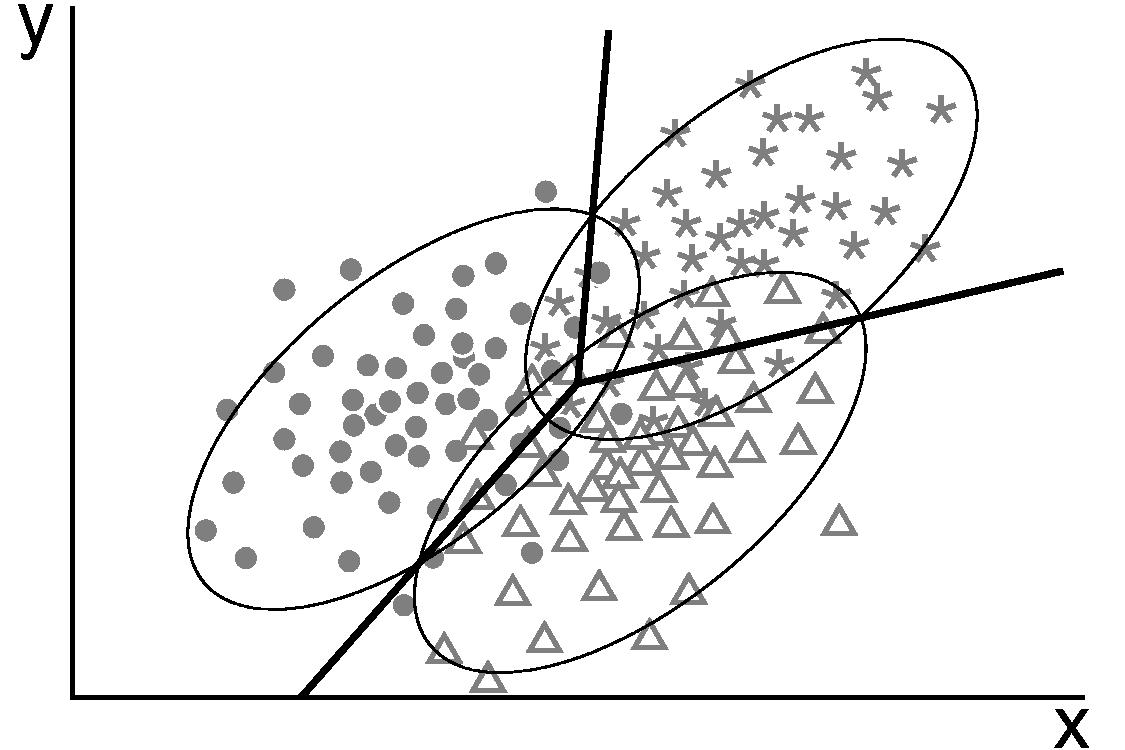
\includegraphics[width=400]{figures/discriminant.jpg}
  \caption[Linear discriminant analysis]{
Discriminant analysis of three  classes with equal covariance matrices
leads to  linear discriminant boundaries. The  ellipses mark arbitrary
(e.g., 95\%) confidence levels for the underlying populations.}
\end{figure}

\begin{figure}[htbp]
  \centering
  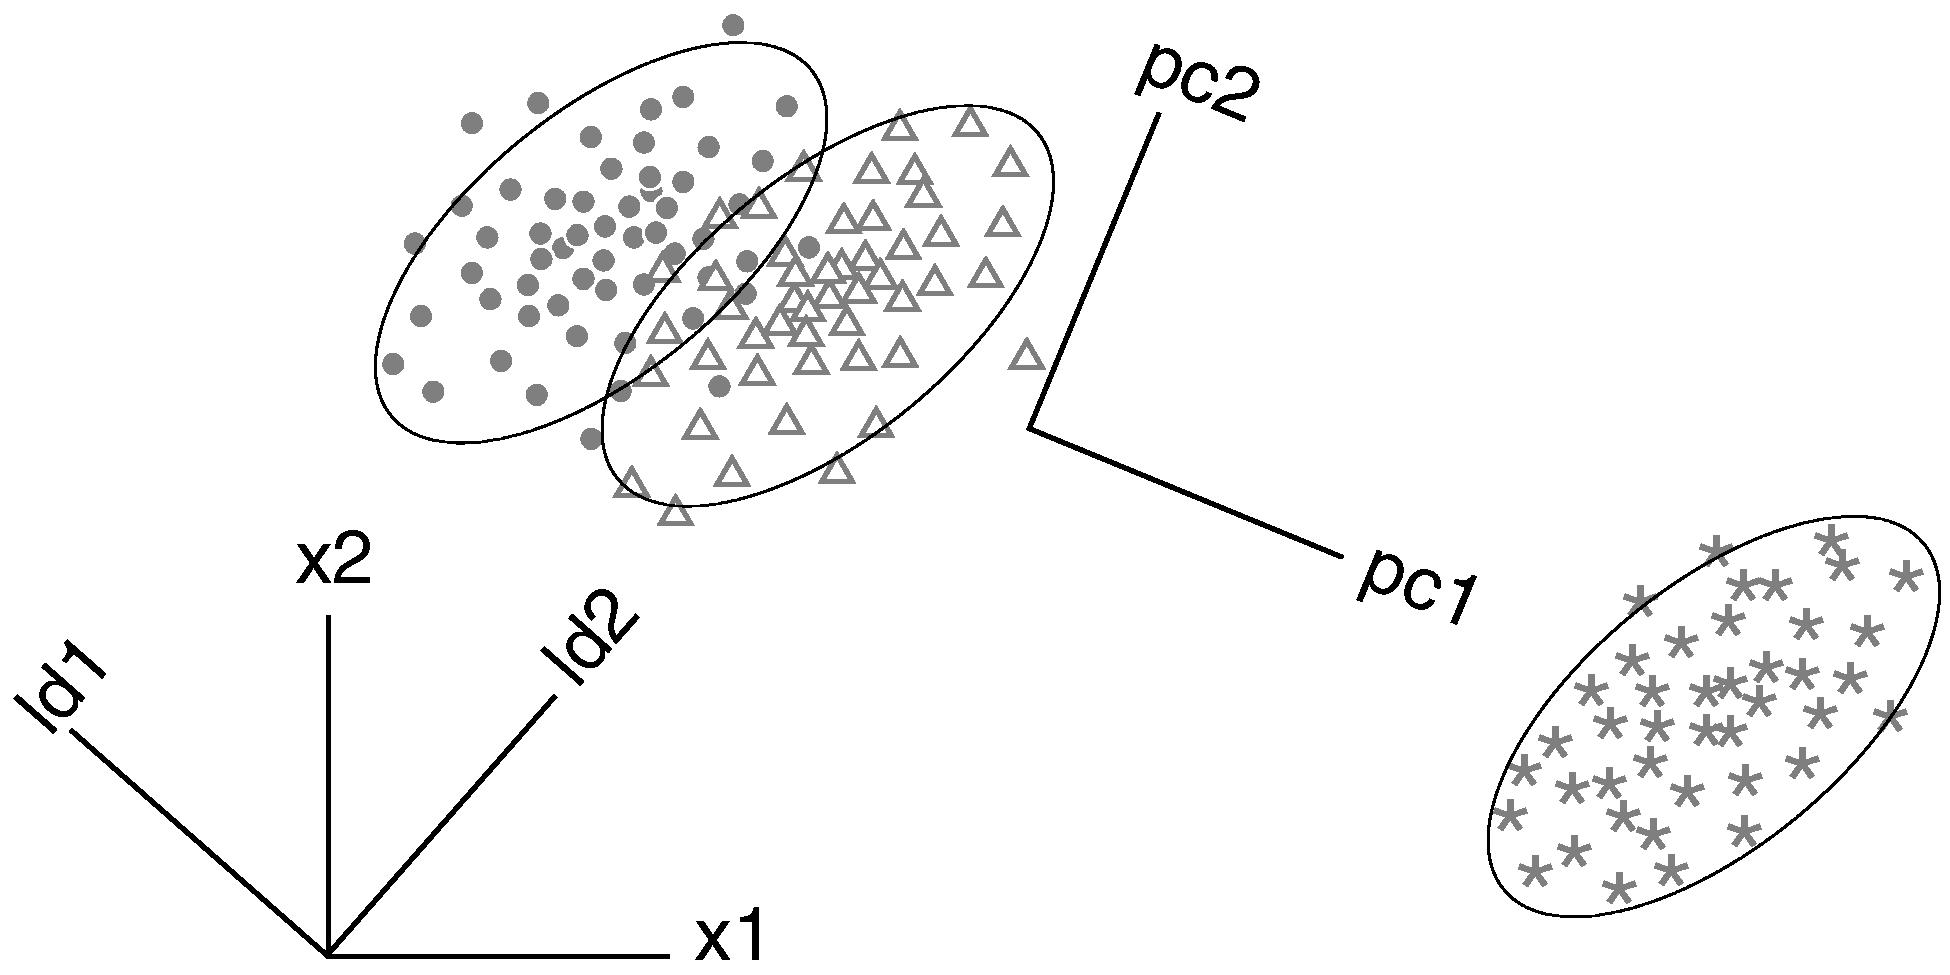
\includegraphics[width=600]{figures/PCAvsLDA.jpg}
  \caption[The difference between PCA and LDA]
{Similarities   and  differences   between  linear   discriminant  and
principal component  analysis.  x1 and x2 are  the original variables,
pc1  and pc2  are the  principal components  and ld1  and ld2  are the
linear discriminant functions.}
  \label{fig:PCAvsLDA}
\end{figure}

\begin{figure}[htbp]
  \centering
  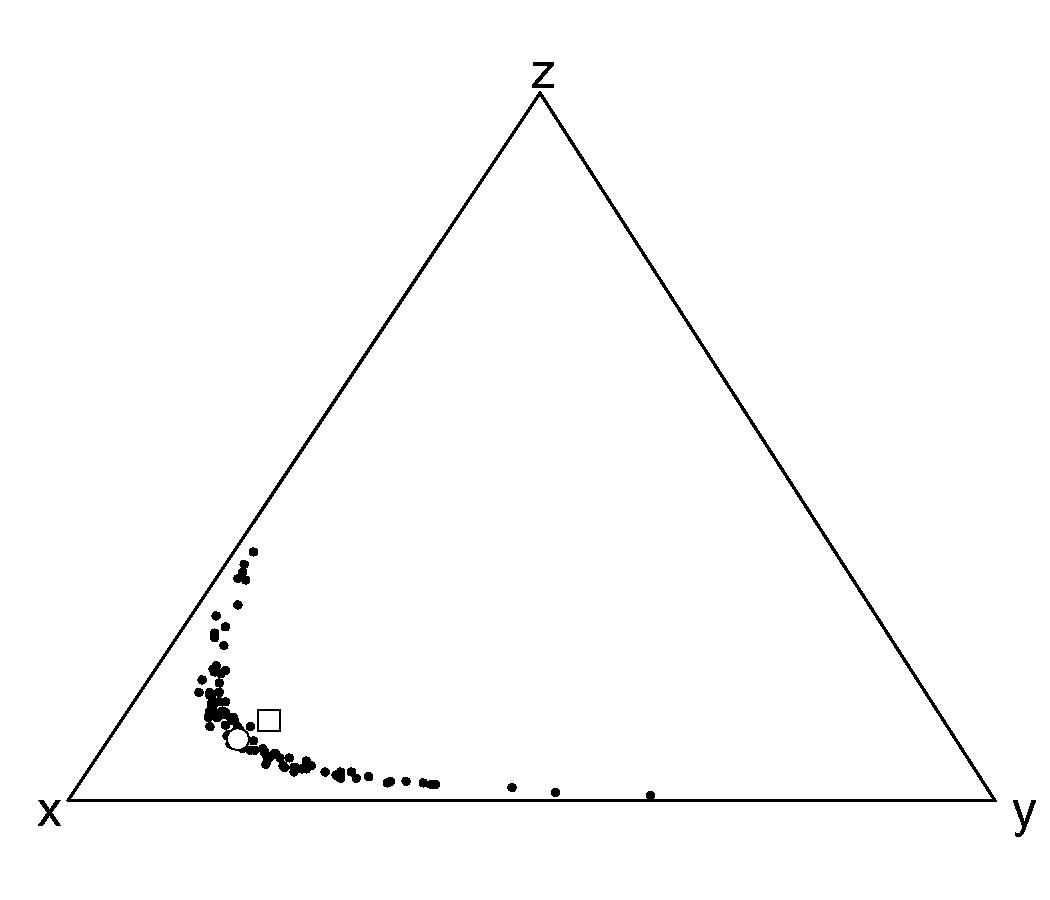
\includegraphics[width=400]{figures/closure.jpg}
  \caption[The consequences of the constant-sum constraint]
{One   of  the   consequences  of   the  constant-sum   constraint  of
compositional data  is that  the arithmetic mean  (marked by  the open
square) of populations (black  dots) has no physical meaning. Instead,
the geometric mean should be used (open circle).}
  \label{fig:closure}
\end{figure}

\begin{figure}[htbp]
  \centering
  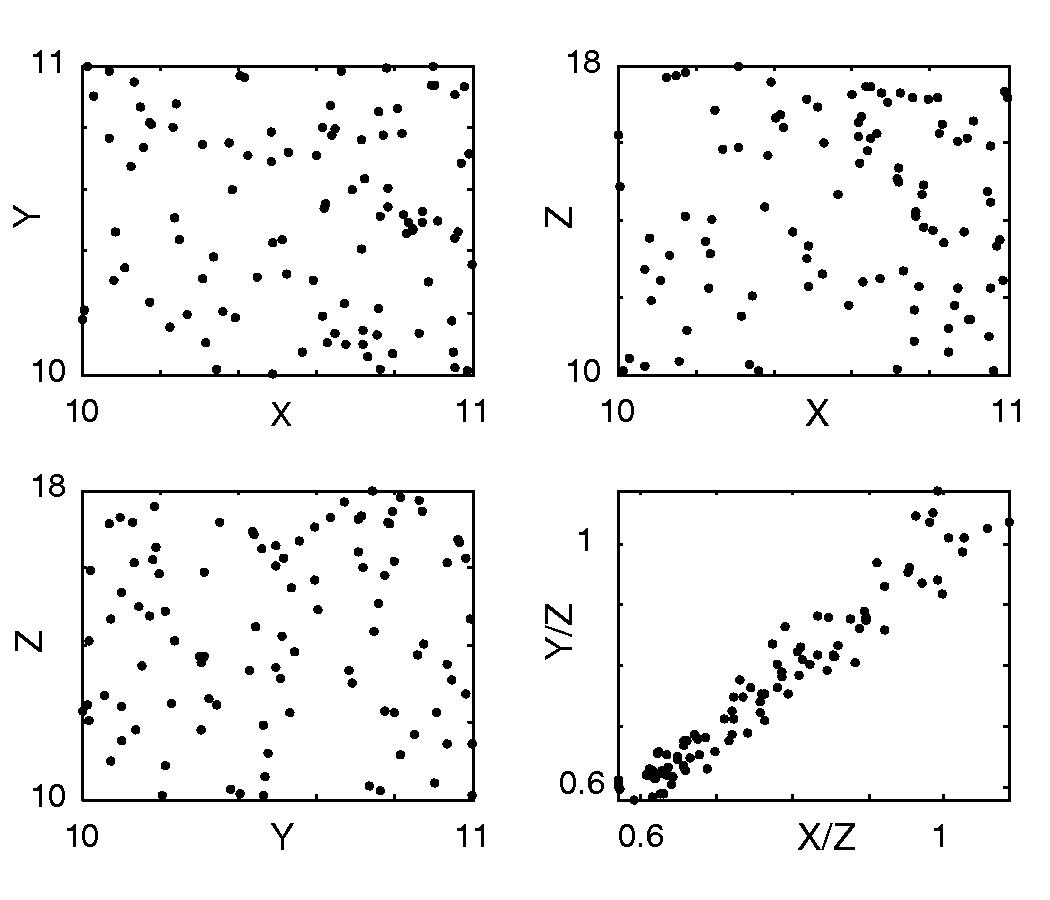
\includegraphics[width=600]{figures/spurious2.jpg}
  \caption[Spurious correlation of ratios]{X, Y and Z are uncorrelated, 
uniform random numbers. The  strong spurious correlation of the ratios
Y/Z  and X/Z  is an  artifact of  the relatively  large variance  of Z
relative to X, Y and Z.}
  \label{fig:spurious}
\end{figure}

\begin{figure}[htbp]
  \centering
  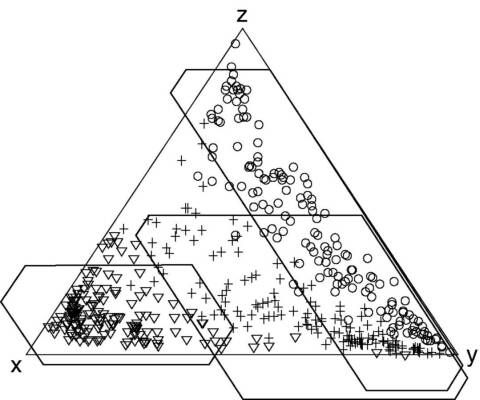
\includegraphics[width=400]{figures/closure_ternary_wrong2.jpg}
  \caption[The dangers of using ``traditional'' statistics on the simplex]{
95\%  normal confidence  regions  (e.g., Weltje,  2002) for  synthetic
trivariate compositional data partly fall outside the ternary diagram,
a   nonsense   result   illustrating   the   dangers   of   performing
``traditional'' statistics on the simplex.}
  \label{fig:closure_ternary_wrong}
\end{figure}

\begin{figure}[htbp]
  \centering
  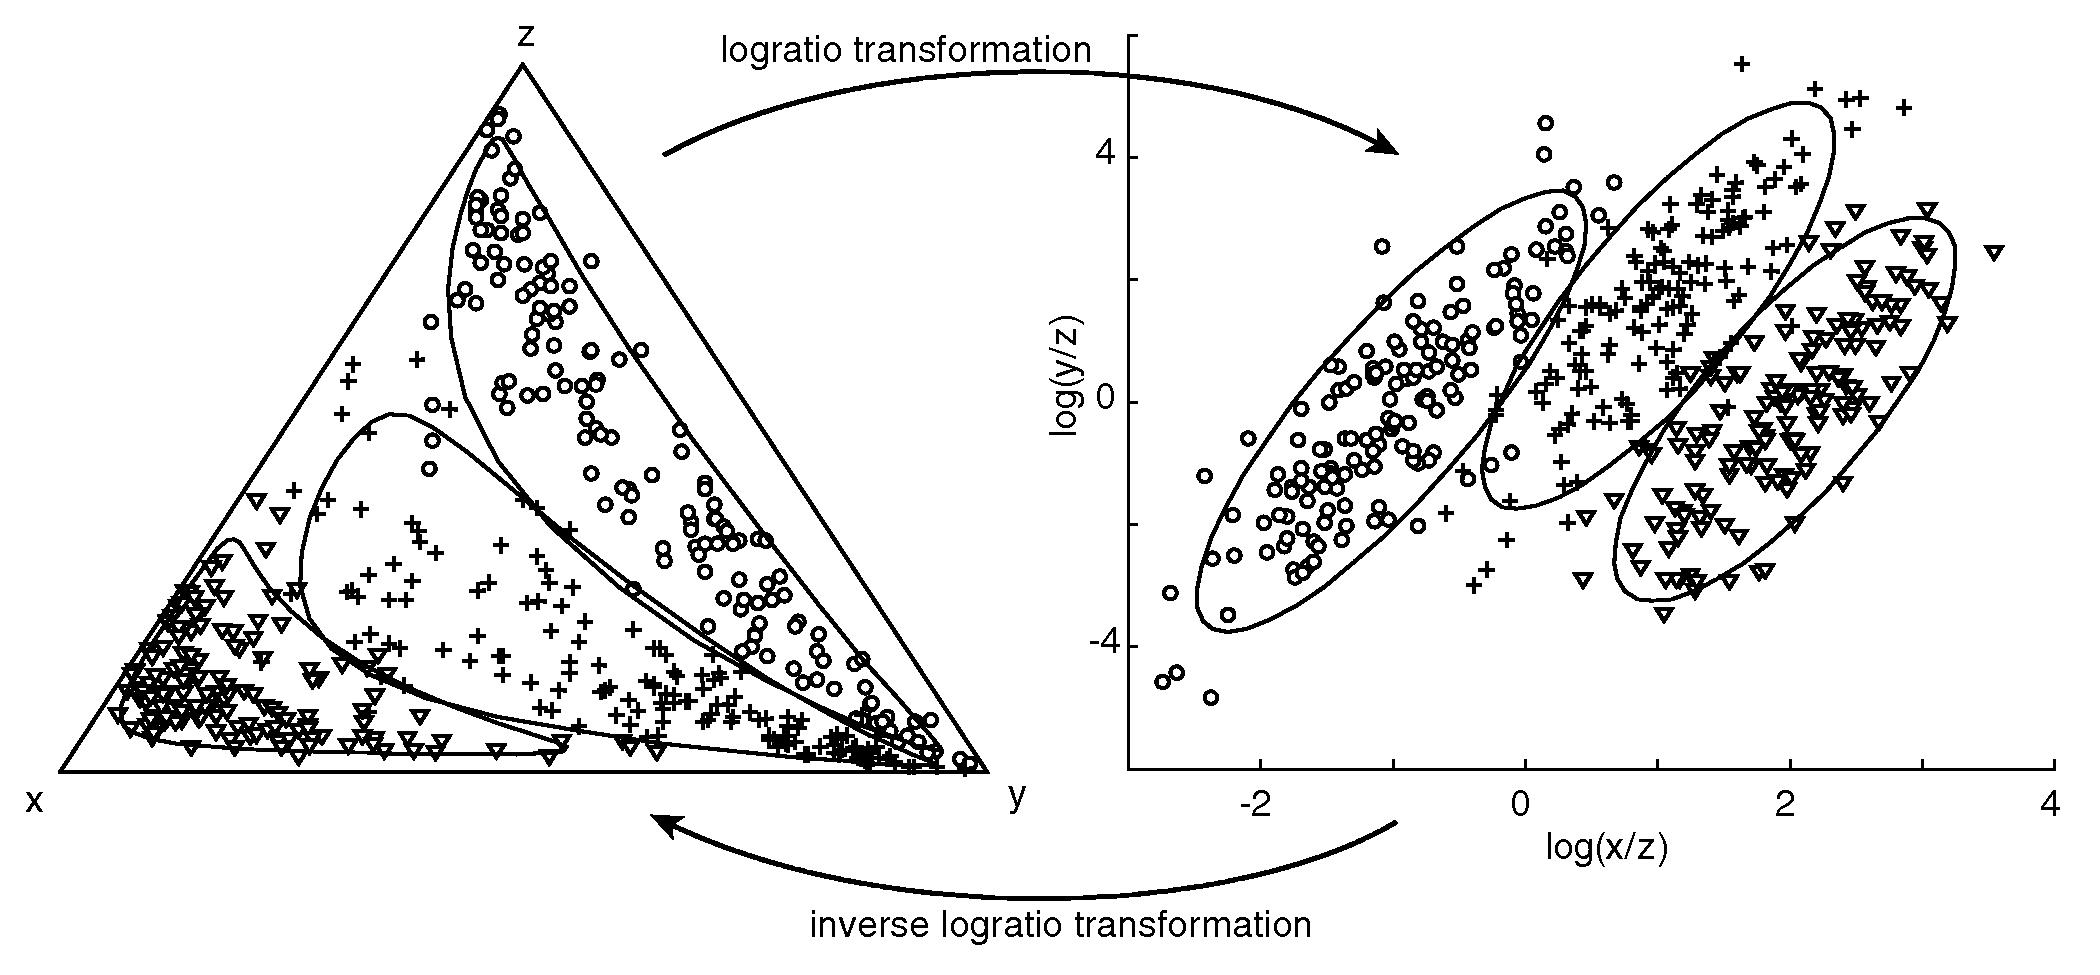
\includegraphics[width=600]{figures/closure_mapping.jpg}
  \caption[Mapping compositional data from $\Delta_2$  to  $\mathbb{R}^2$]{
Following  Aitchison  (1986),   the  statistical  problems  of  Figure
\ref{fig:closure_ternary_wrong}  can be  avoided by  mapping  the data
from  the  simplex $\Delta_2$  to  $\mathbb{R}^2$  using the  logratio
transformation.}
  \label{fig:closure_mapping}
\end{figure}

\begin{figure}[htbp]
  \centering
  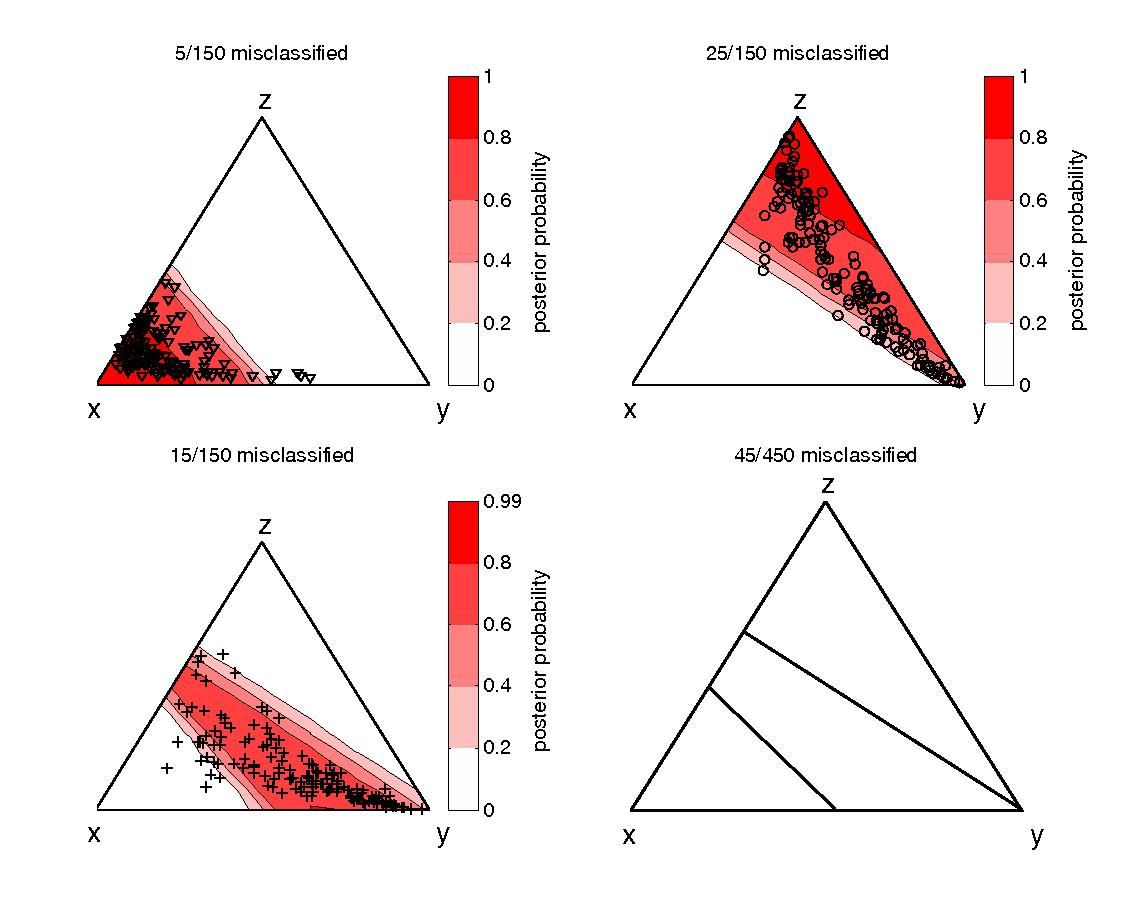
\includegraphics[width=600]{figures/closure_discriminant_wrong.jpg}
  \caption[Linear discriminant analysis done the wrong way]{
Linear discriminant analysis using the {\it crude covariance} approach
of Figure \ref{fig:closure_ternary_wrong}.  The red-shaded contours of
the first three ternary diagrams represent the posterior probabilities
for the  three classes.   The last diagram  shows the  linear decision
boundaries. 10\% of the training data are misclassified.}
  \label{fig:closure_discriminant_wrong}
\end{figure}

\begin{figure}[htbp]
  \centering
  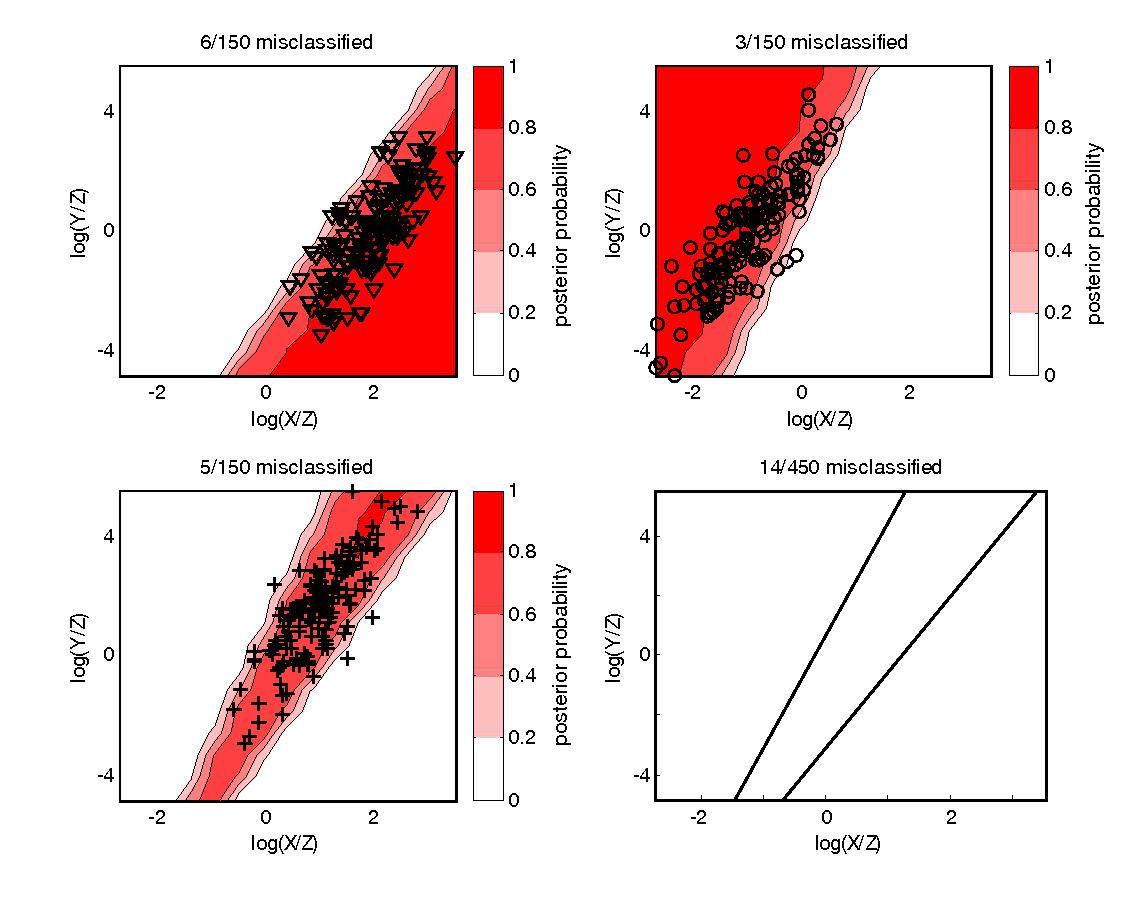
\includegraphics[width=600]{figures/closure_binary_discriminant_right.jpg}
\caption[Linear discriminant analysis done the right way]{
The same  data of Figure  \ref{fig:closure_discriminant_wrong}, mapped
to   logratio-space   using  the   approach   illustrated  by   Figure
\ref{fig:closure_mapping}.  Linear   discriminant  analysis  of  these
bivariate data misclassifies only 3\% of the training data.}
  \label{fig:closure_binary_discriminant_right}
\end{figure}

\begin{figure}[htbp]
  \centering
  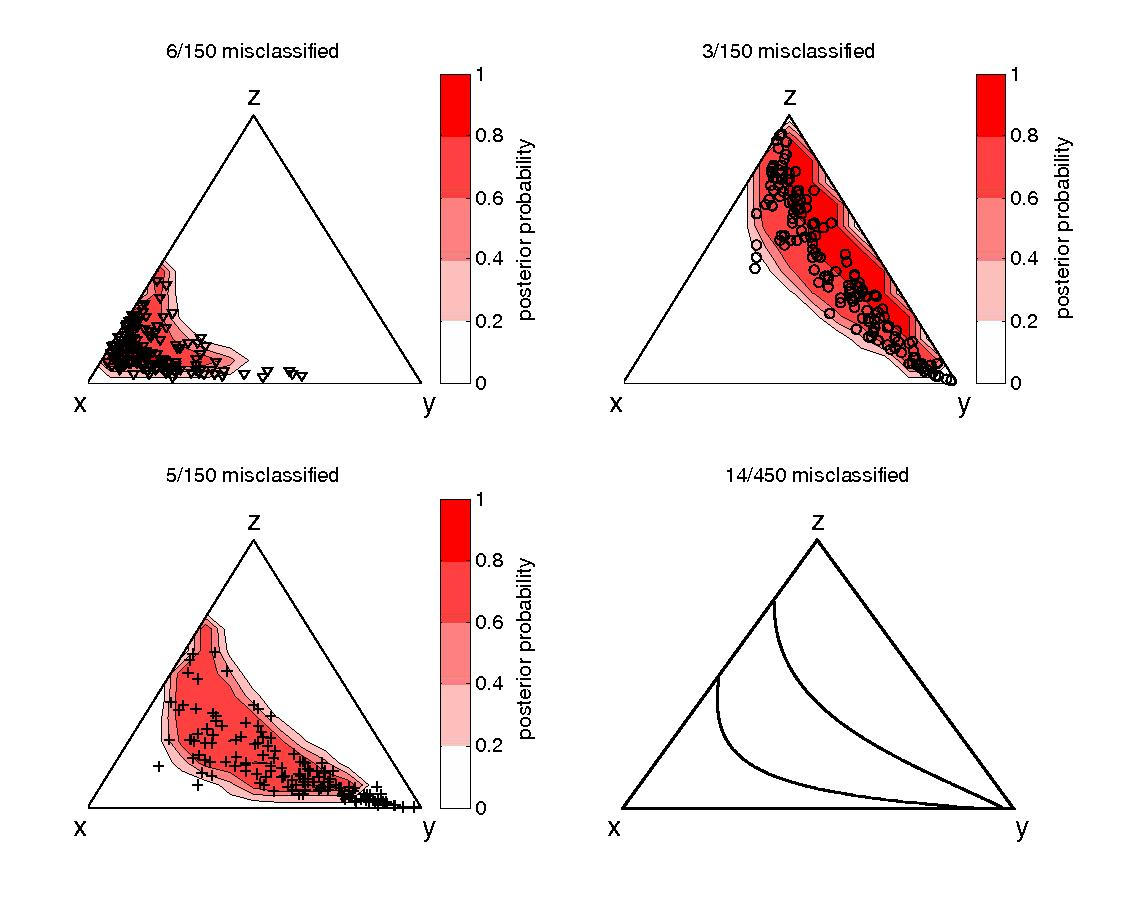
\includegraphics[width=600]{figures/closure_ternary_discriminant_right.jpg}
  \caption[Results of the linear discriminant analysis mapped back to the simplex]{
Mapping the  results of Figure \ref{fig:closure_binary_discriminant_right} 
back  to the ternary  diagram with  the  inverse logratio  transformation shown  on
Figure \ref{fig:closure_mapping} yields curved posterior densities and
decision boundaries.}
  \label{fig:closure_ternary_discriminant_right}
\end{figure}

\begin{figure}[htbp]
  \centering
  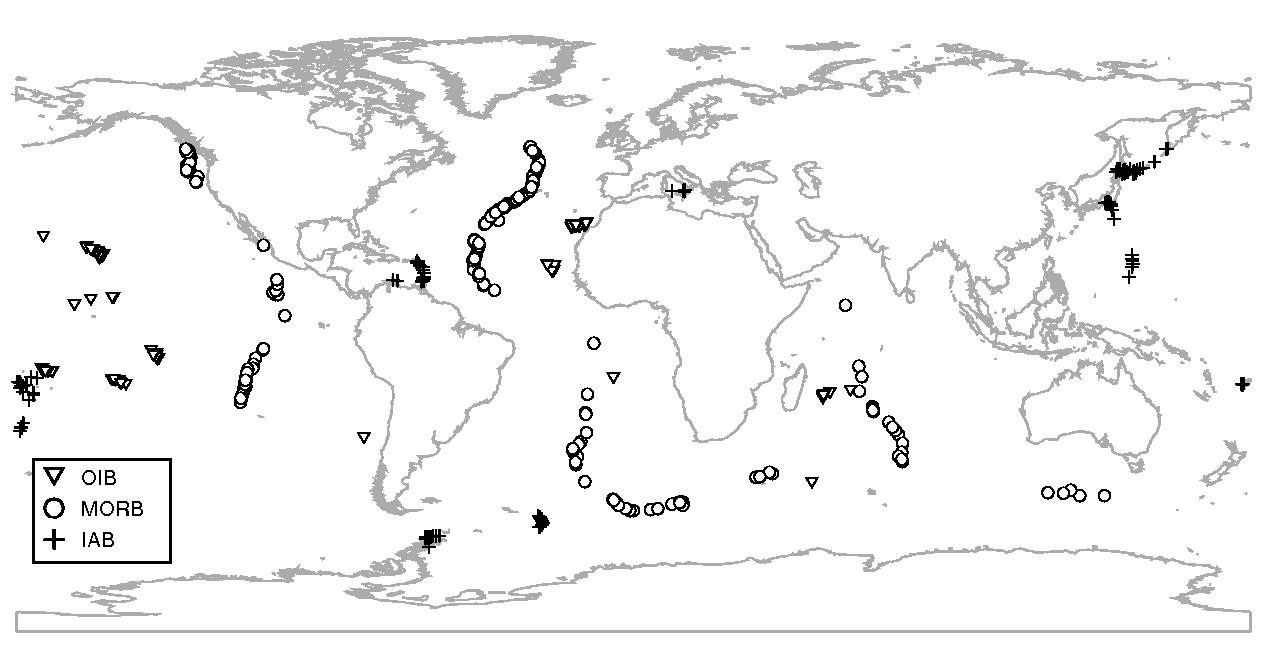
\includegraphics[width=600]{figures/sample_locations.jpg}
  \caption[Geographical locations of the training data]{
Locations of the training data:  756 Island Arc (IAB), Mid Ocean Ridge
(MORB) and Ocean Island (OIB) Basalts.}
  \label{fig:sample_locations}
\end{figure}

\clearpage

\begin{figure}[htbp]
  \centering
  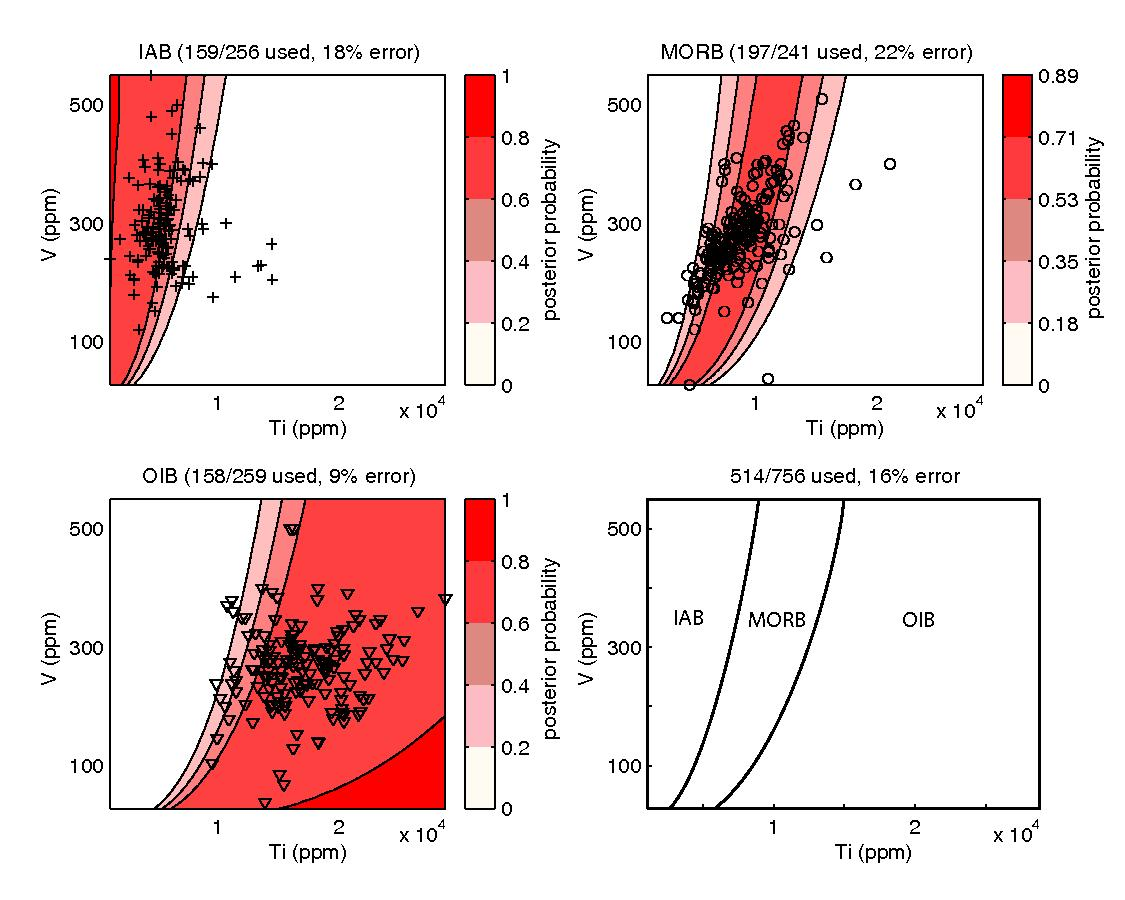
\includegraphics[width=600]{figures/Ti_V_lin.jpg}
  \caption[Linear discriminant analysis of the Ti-V system of Shervais (1982)]
{Linear  discriminant analysis (LDA)  of the  Ti-V system  of Shervais
(1982).  The red-shaded contours on  the first three subplots show the
posterior probability  of a particular  ``class'' (IAB, MORB,  or OIB)
given the training set of 756  basalt samples and a uniform prior. The
last  subplot (lower-right)  shows the  new decision  boundaries.  The
number of training  data used and a resubstitution  error estimate are
given for each of the tectonic affinities.  The overall resubstitution
error is shown above the lower-right subplot.}
  \label{fig:Ti_V_lin}
\end{figure}

\begin{figure}[htbp]
  \centering
  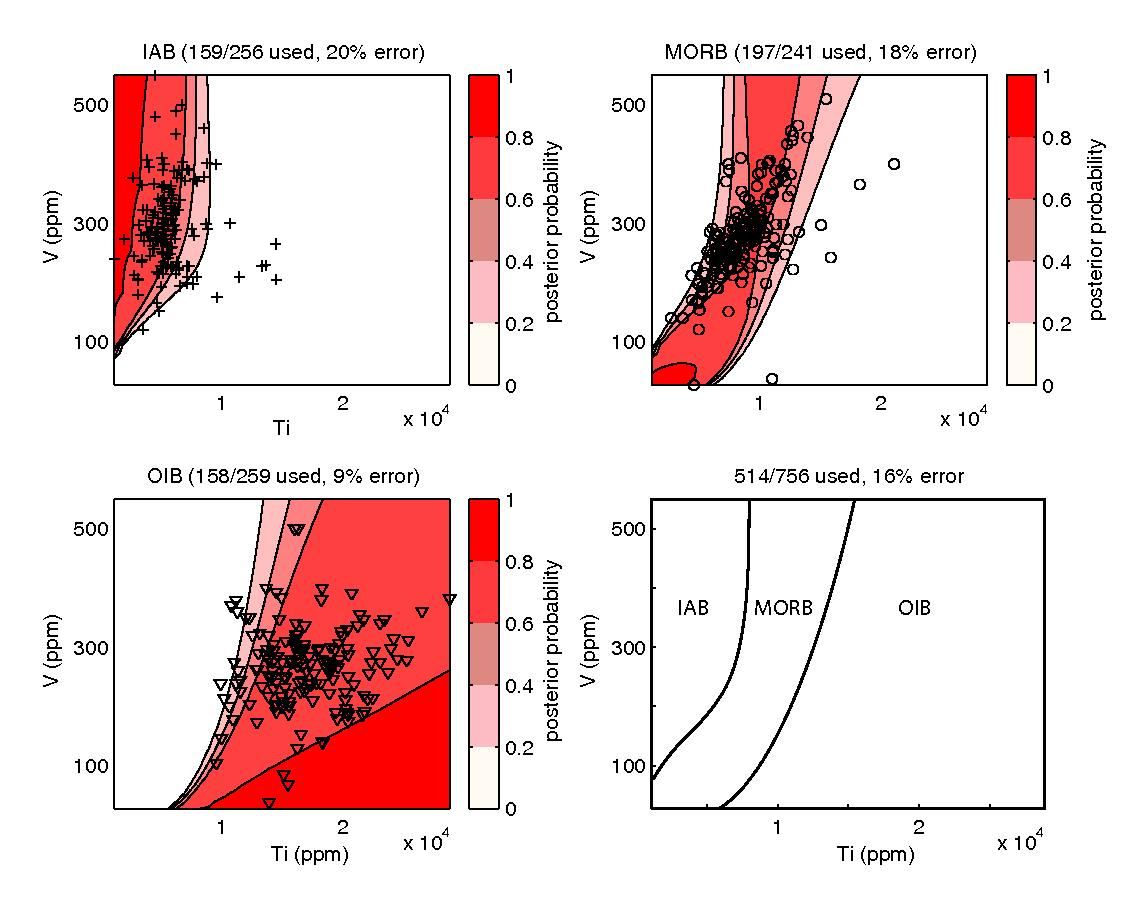
\includegraphics[width=600]{figures/Ti_V_quad.jpg}
  \caption[Quadratic discriminant analysis of the Ti-V system]
{Quadratic discriminant analysis (QDA) of the Ti-V system. In contrast
with the LDA of Figure \ref{fig:Ti_V_lin}, each tectonic ``class'' was
allowed to  have a different covariance matrix,  resulting in slightly
different decision boundaries.}
  \label{fig:Ti_V_quad}
\end{figure}

\begin{figure}[htbp]
  \centering
  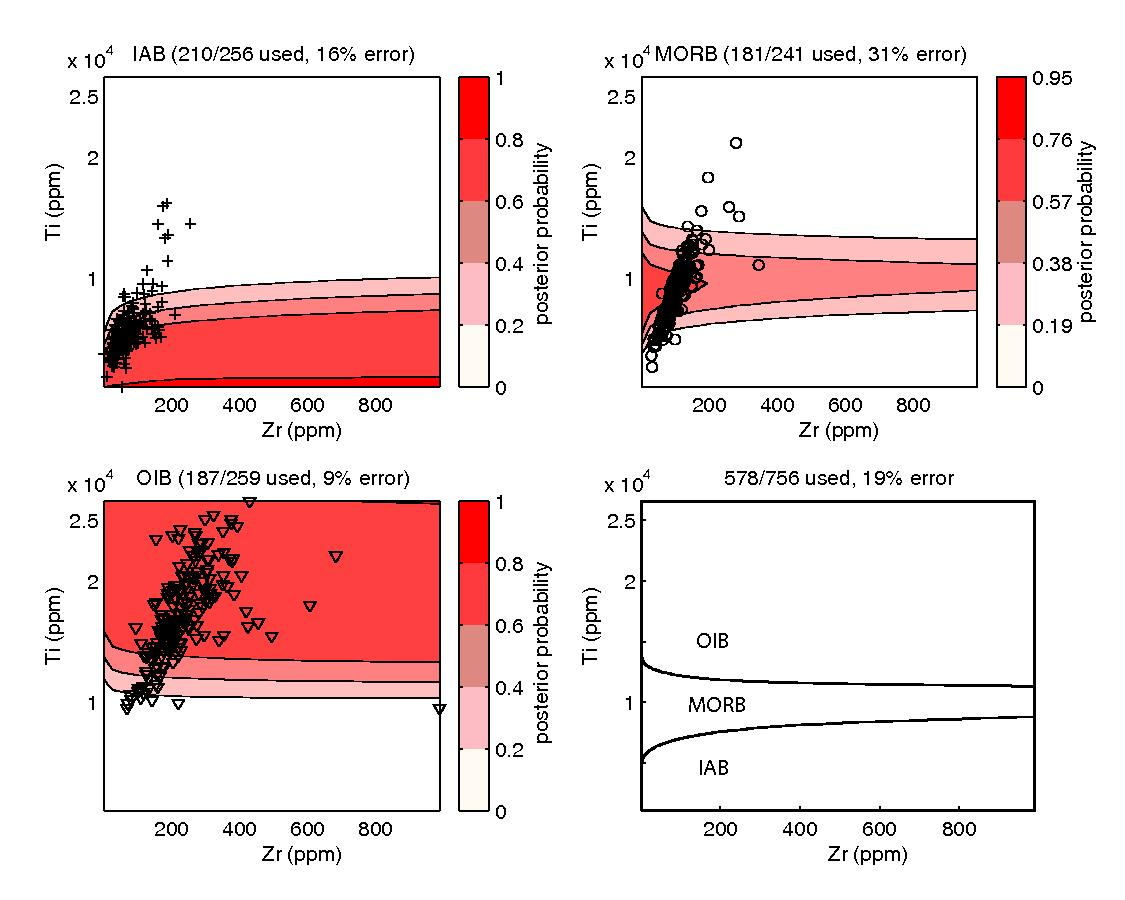
\includegraphics[width=600]{figures/Ti_Zr_lin.jpg}
  \caption[Linear discriminant analysis of the Ti-Zr system of Pearce and Cann (1973)]
{Linear discriminant analysis of the Ti-Zr system of Pearce and Cann (1973).}
  \label{fig:Ti_Zr_lin}
\end{figure}

\begin{figure}[htbp]
  \centering
  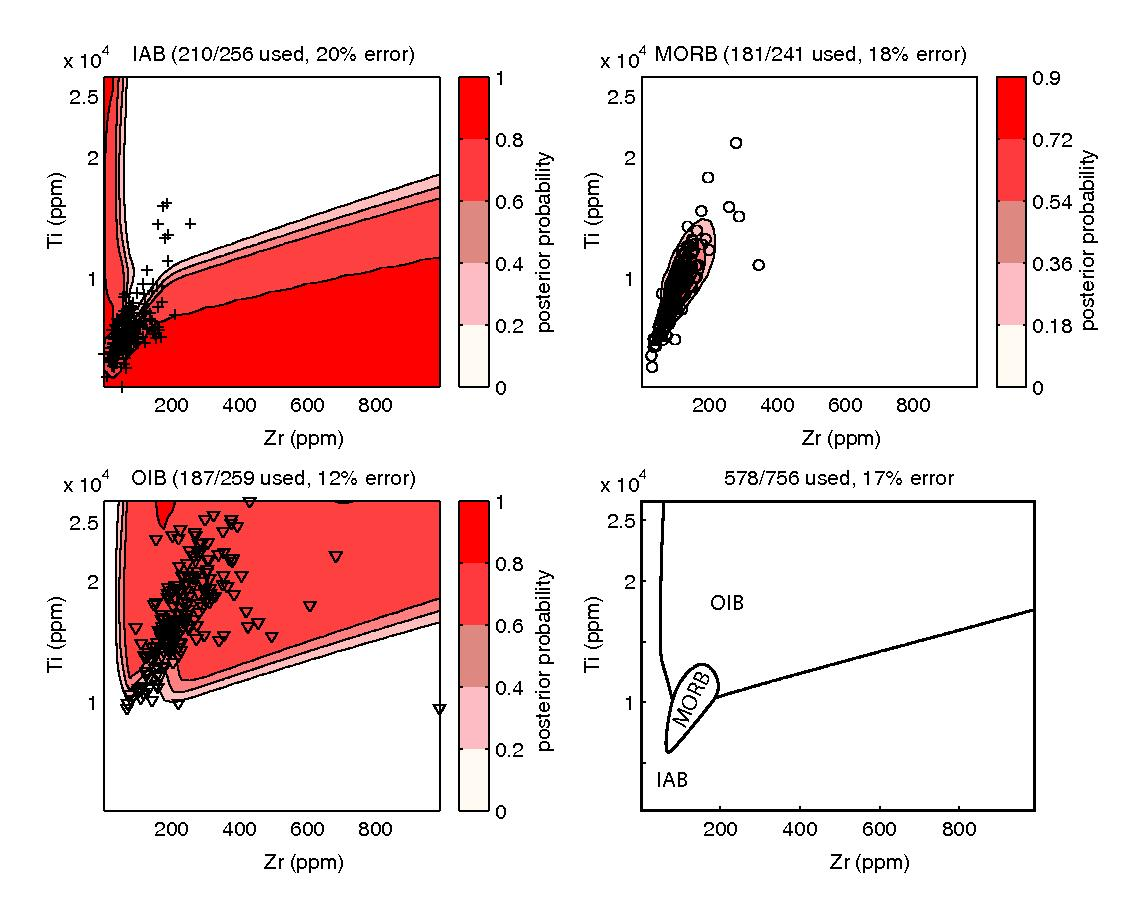
\includegraphics[width=600]{figures/Ti_Zr_quad.jpg}
  \caption[Quadratic discriminant analysis of the Ti-Zr system]
{Quadratic discriminant analysis of the Ti-Zr system.}
  \label{fig:Ti_Zr_quad}
\end{figure}

\begin{figure}[htbp]
  \centering
  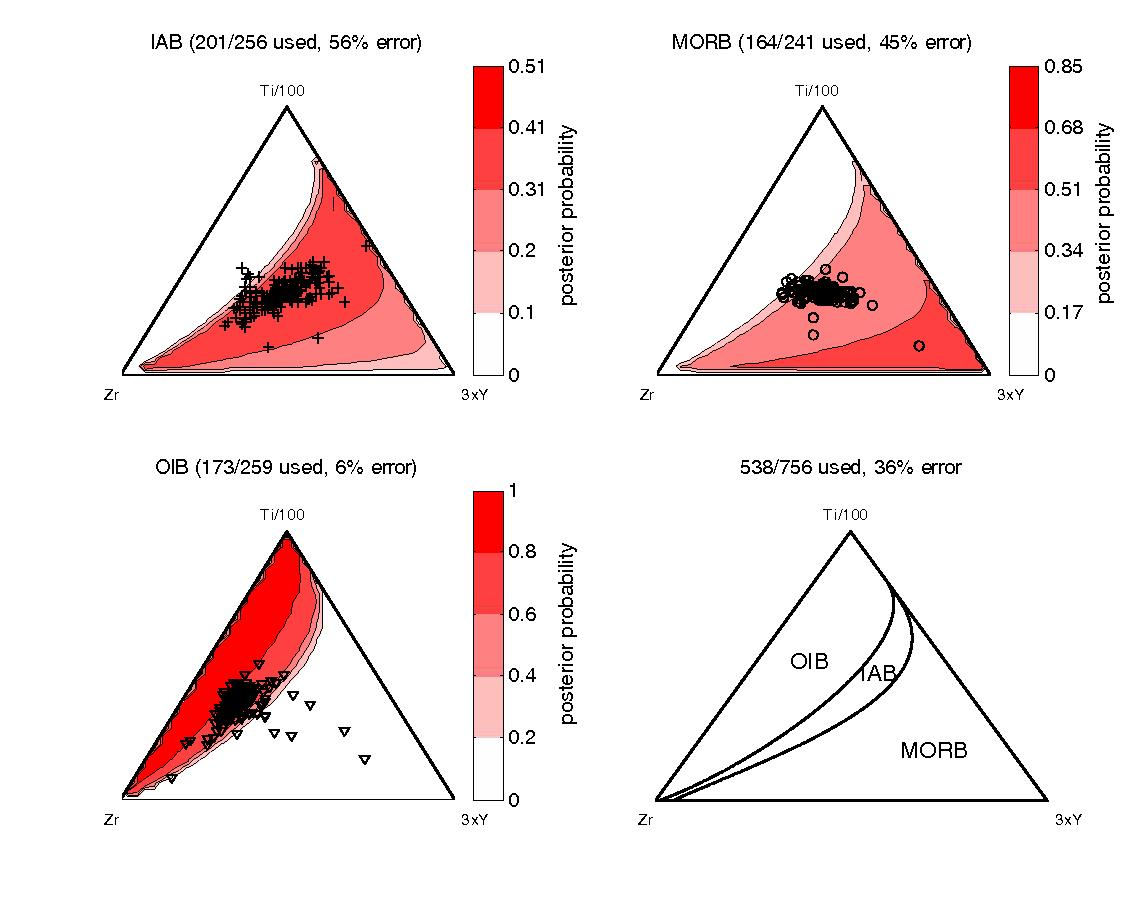
\includegraphics[width=600]{figures/Ti_Zr_Y_lin.jpg}
  \caption[Linear discriminant analysis of the Ti-Zr-Y system of Pearce and Cann (1973)]
{Linear discriminant analysis of the Ti-Zr-Y system of Pearce and Cann
(1973).  The  posterior probabilities of  nearly all the IAB  and MORB
training data  are low ($<$0.4), resulting  in large misclassification
rates for  these affinities. As noted  by Pearce and  Cann (1973), the
Ti-Zr-Y  diagram can  be used  to  separate OIBs  from IAB/MORBs,  but
cannot be used to distinguish  between IAB and MORB. For this purpose,
the Ti-Zr diagram (Figure \ref{fig:Ti_Zr_lin}) can be used.}
  \label{fig:Ti_Zr_Y_lin}
\end{figure}

\begin{figure}[htbp]
  \centering
  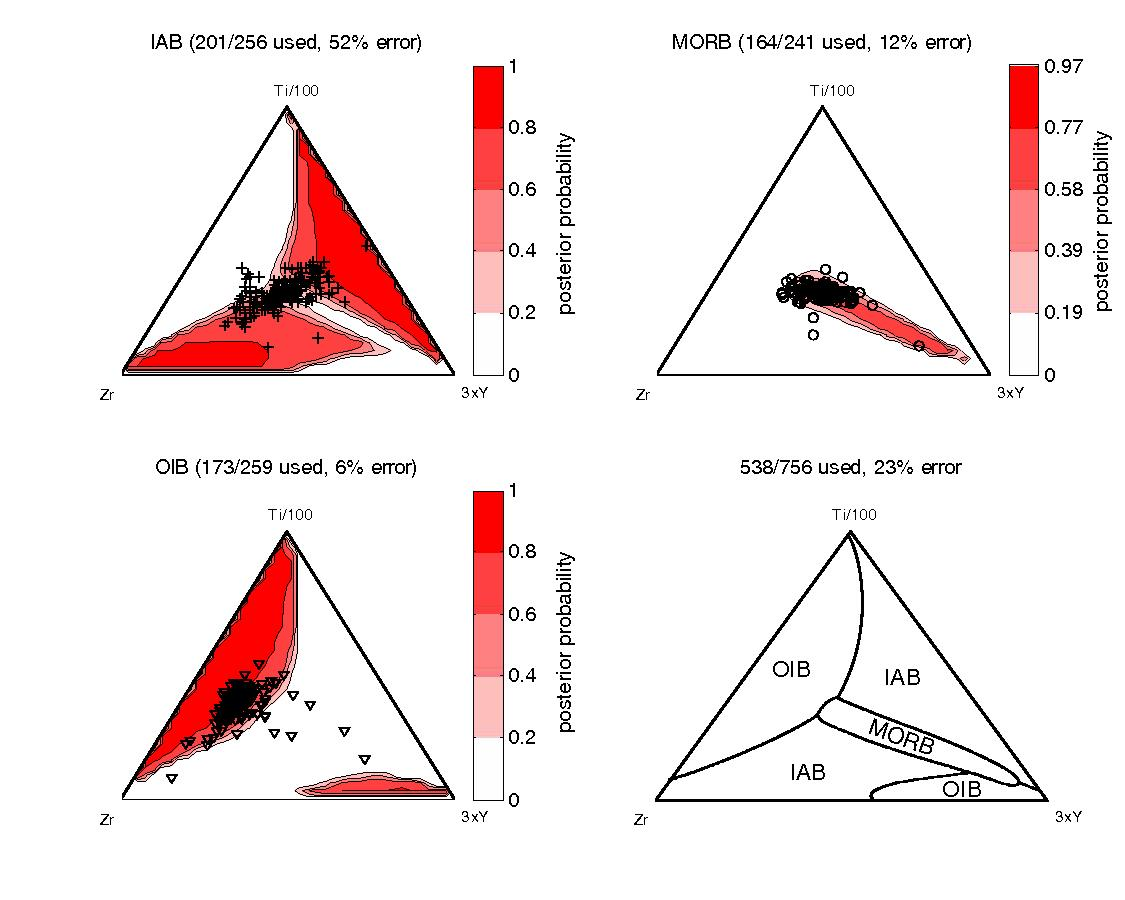
\includegraphics[width=600]{figures/Ti_Zr_Y_quad.jpg}
  \caption[Quadratic discriminant analysis of the Ti-Zr-Y system]
{Quadratic discriminant  analysis of the Ti-Zr-Y  system.  The OIB/IAB
decision boundary  (at low  Y) is nearly  identical to that  of Figure
\ref{fig:Ti_Zr_Y_lin},  whereas   there  is  a   lot  more  (unstable)
structure at higher Y concentrations.}
  \label{fig:Ti_Zr_Y_quad}
\end{figure}

\begin{figure}[htbp]
  \centering
  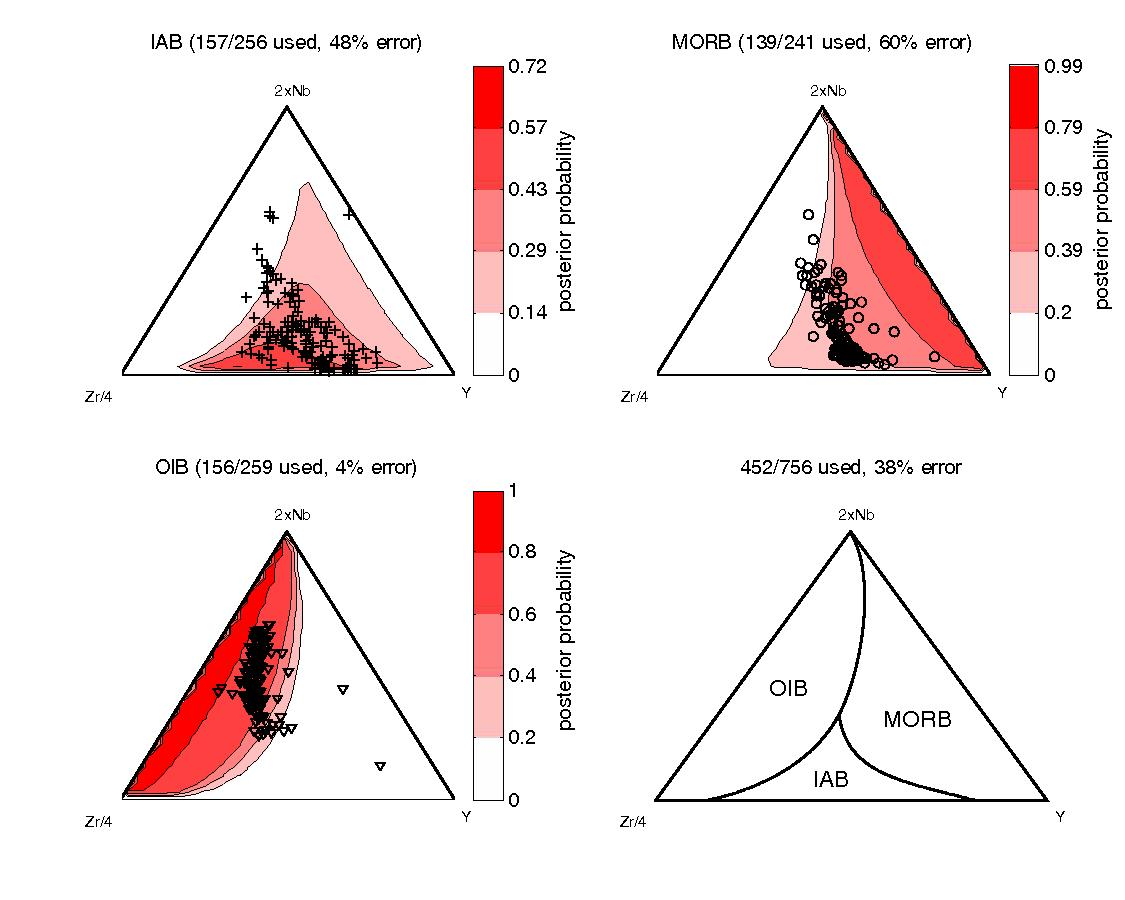
\includegraphics[width=600]{figures/Nb_Zr_Y_lin.jpg}
  \caption[Linear discriminant analysis of the Zr-Y-Nb system of Meschede (1986)]
{Linear  discriminant  analysis  of  the Zr-Y-Nb  system  of  Meschede
(1986). Like  in Figure \ref{fig:Ti_Zr_Y_lin}, posterior  IAB and MORB
probabilities are low, resulting in high misclassification rates.}
  \label{fig:Nb_Zr_Y_lin}
\end{figure}

\begin{figure}[htbp]
  \centering
  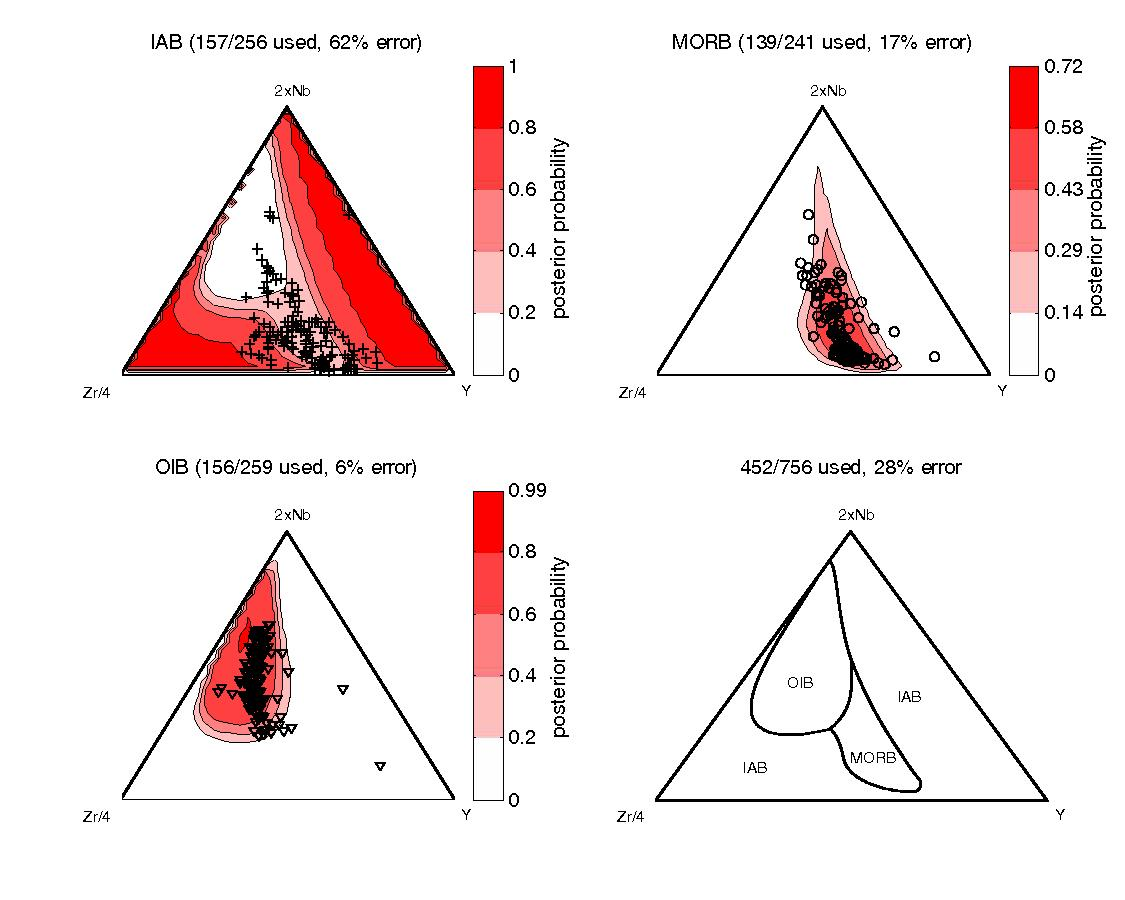
\includegraphics[width=600]{figures/Nb_Zr_Y_quad.jpg}
  \caption[Quadratic discriminant analysis of the Zr-Y-Nb system]
{Quadratic discriminant analysis of the Zr-Y-Nb system.}
  \label{fig:Nb_Zr_Y_quad}
\end{figure}

\begin{figure}[htbp]
  \centering
  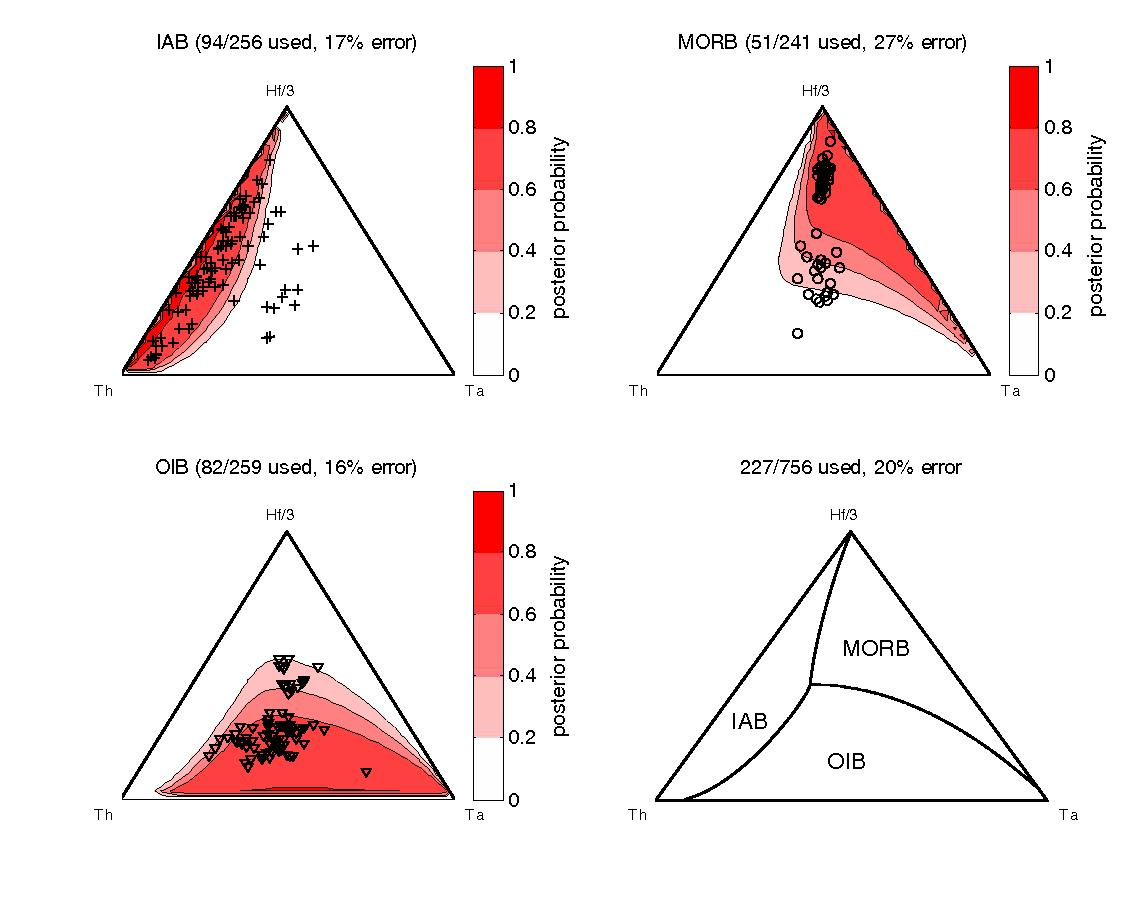
\includegraphics[width=600]{figures/Th_Ta_Hf_lin.jpg}
  \caption[Linear discriminant analysis of the Th-Ta-Hf system of Wood (1980)]
{Linear discriminant analysis of the Th-Ta-Hf system of Wood (1980).}
  \label{fig:Th_Ta_Hf_lin}
\end{figure}

\begin{figure}[htbp]
  \centering
  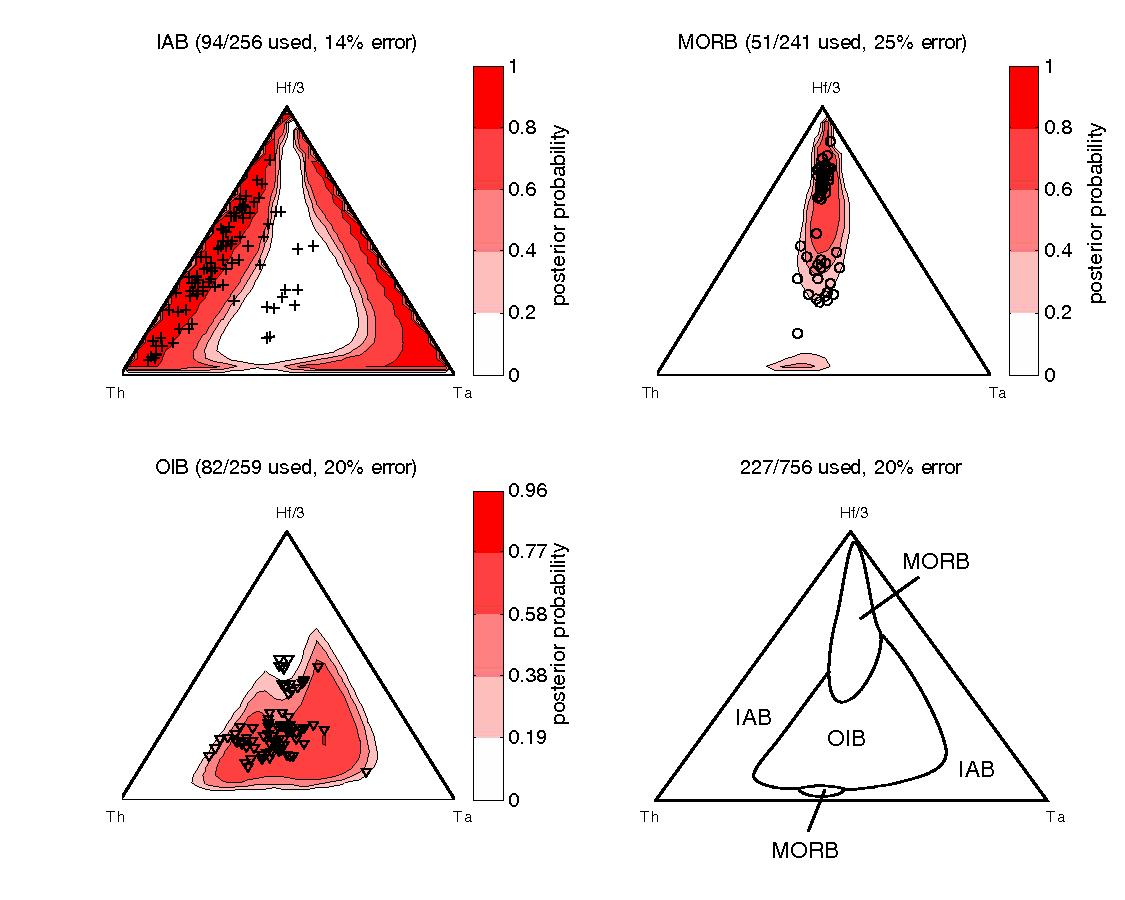
\includegraphics[width=600]{figures/Th_Ta_Hf_quad.jpg}
  \caption[Quadratic discriminant analysis of the Th-Ta-Hf system]
{Quadratic discriminant analysis of the Th-Ta-Hf system.}
  \label{fig:Th_Ta_Hf_quad}
\end{figure}

\clearpage

\begin{figure}[htbp]
  \centering
  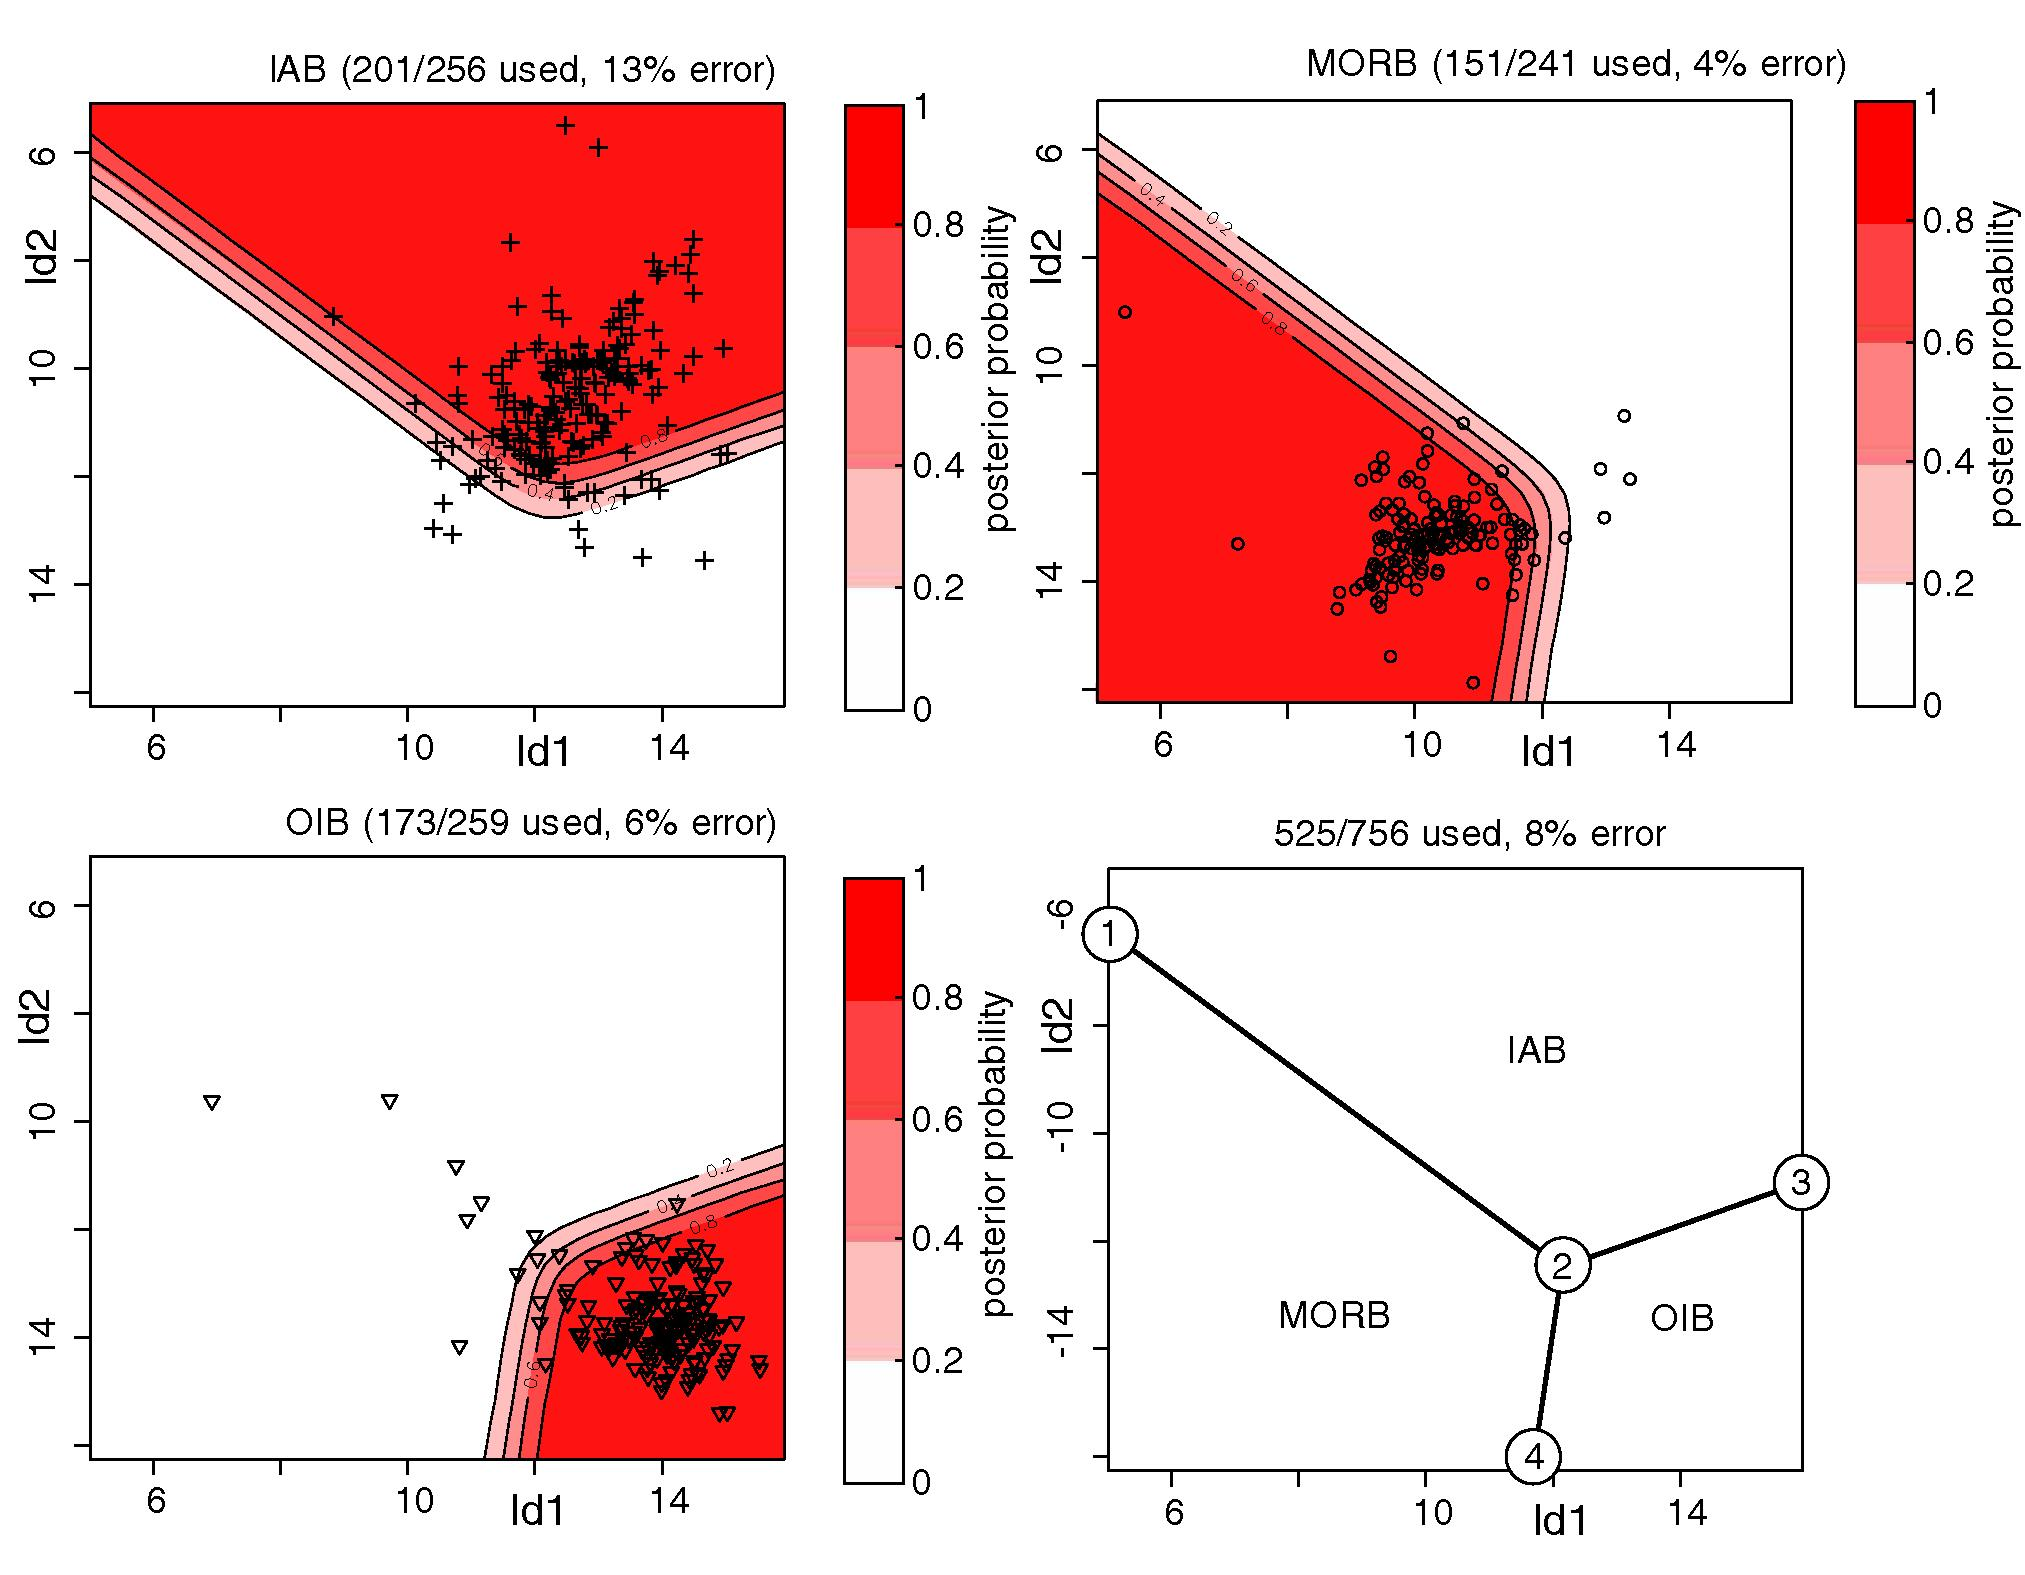
\includegraphics[width=600]{figures/discrimiFunc2.jpg}
  \caption[Linear discriminant analysis using Ti, Zr, Y and Sr]{
Linear discriminant analysis of the Ti-Zr-Y-Sr system. ld1 and ld2 are
the   two   linear   discriminant   functions,   given   by   Equation
\ref{eq:ld_a}.   They represent two  projection planes  that optimally
separate the three tectonic affinities  (IAB, MORB, and OIB) (see also
Figure \ref{fig:PCAvsLDA}).  The encircled  numbers on the lower right
subplot  are  ``anchor  points'' that  can  be  used  by the  user  to
reconstruct  the decision boundaries  in logratio-space.   The ld1/ld2
coordinates   of   these   anchor    points   are   given   in   Table
\ref{tab:anchors}.}
  \label{fig:discrimiFunc1}
\end{figure}

\begin{figure}[htbp]
  \centering
  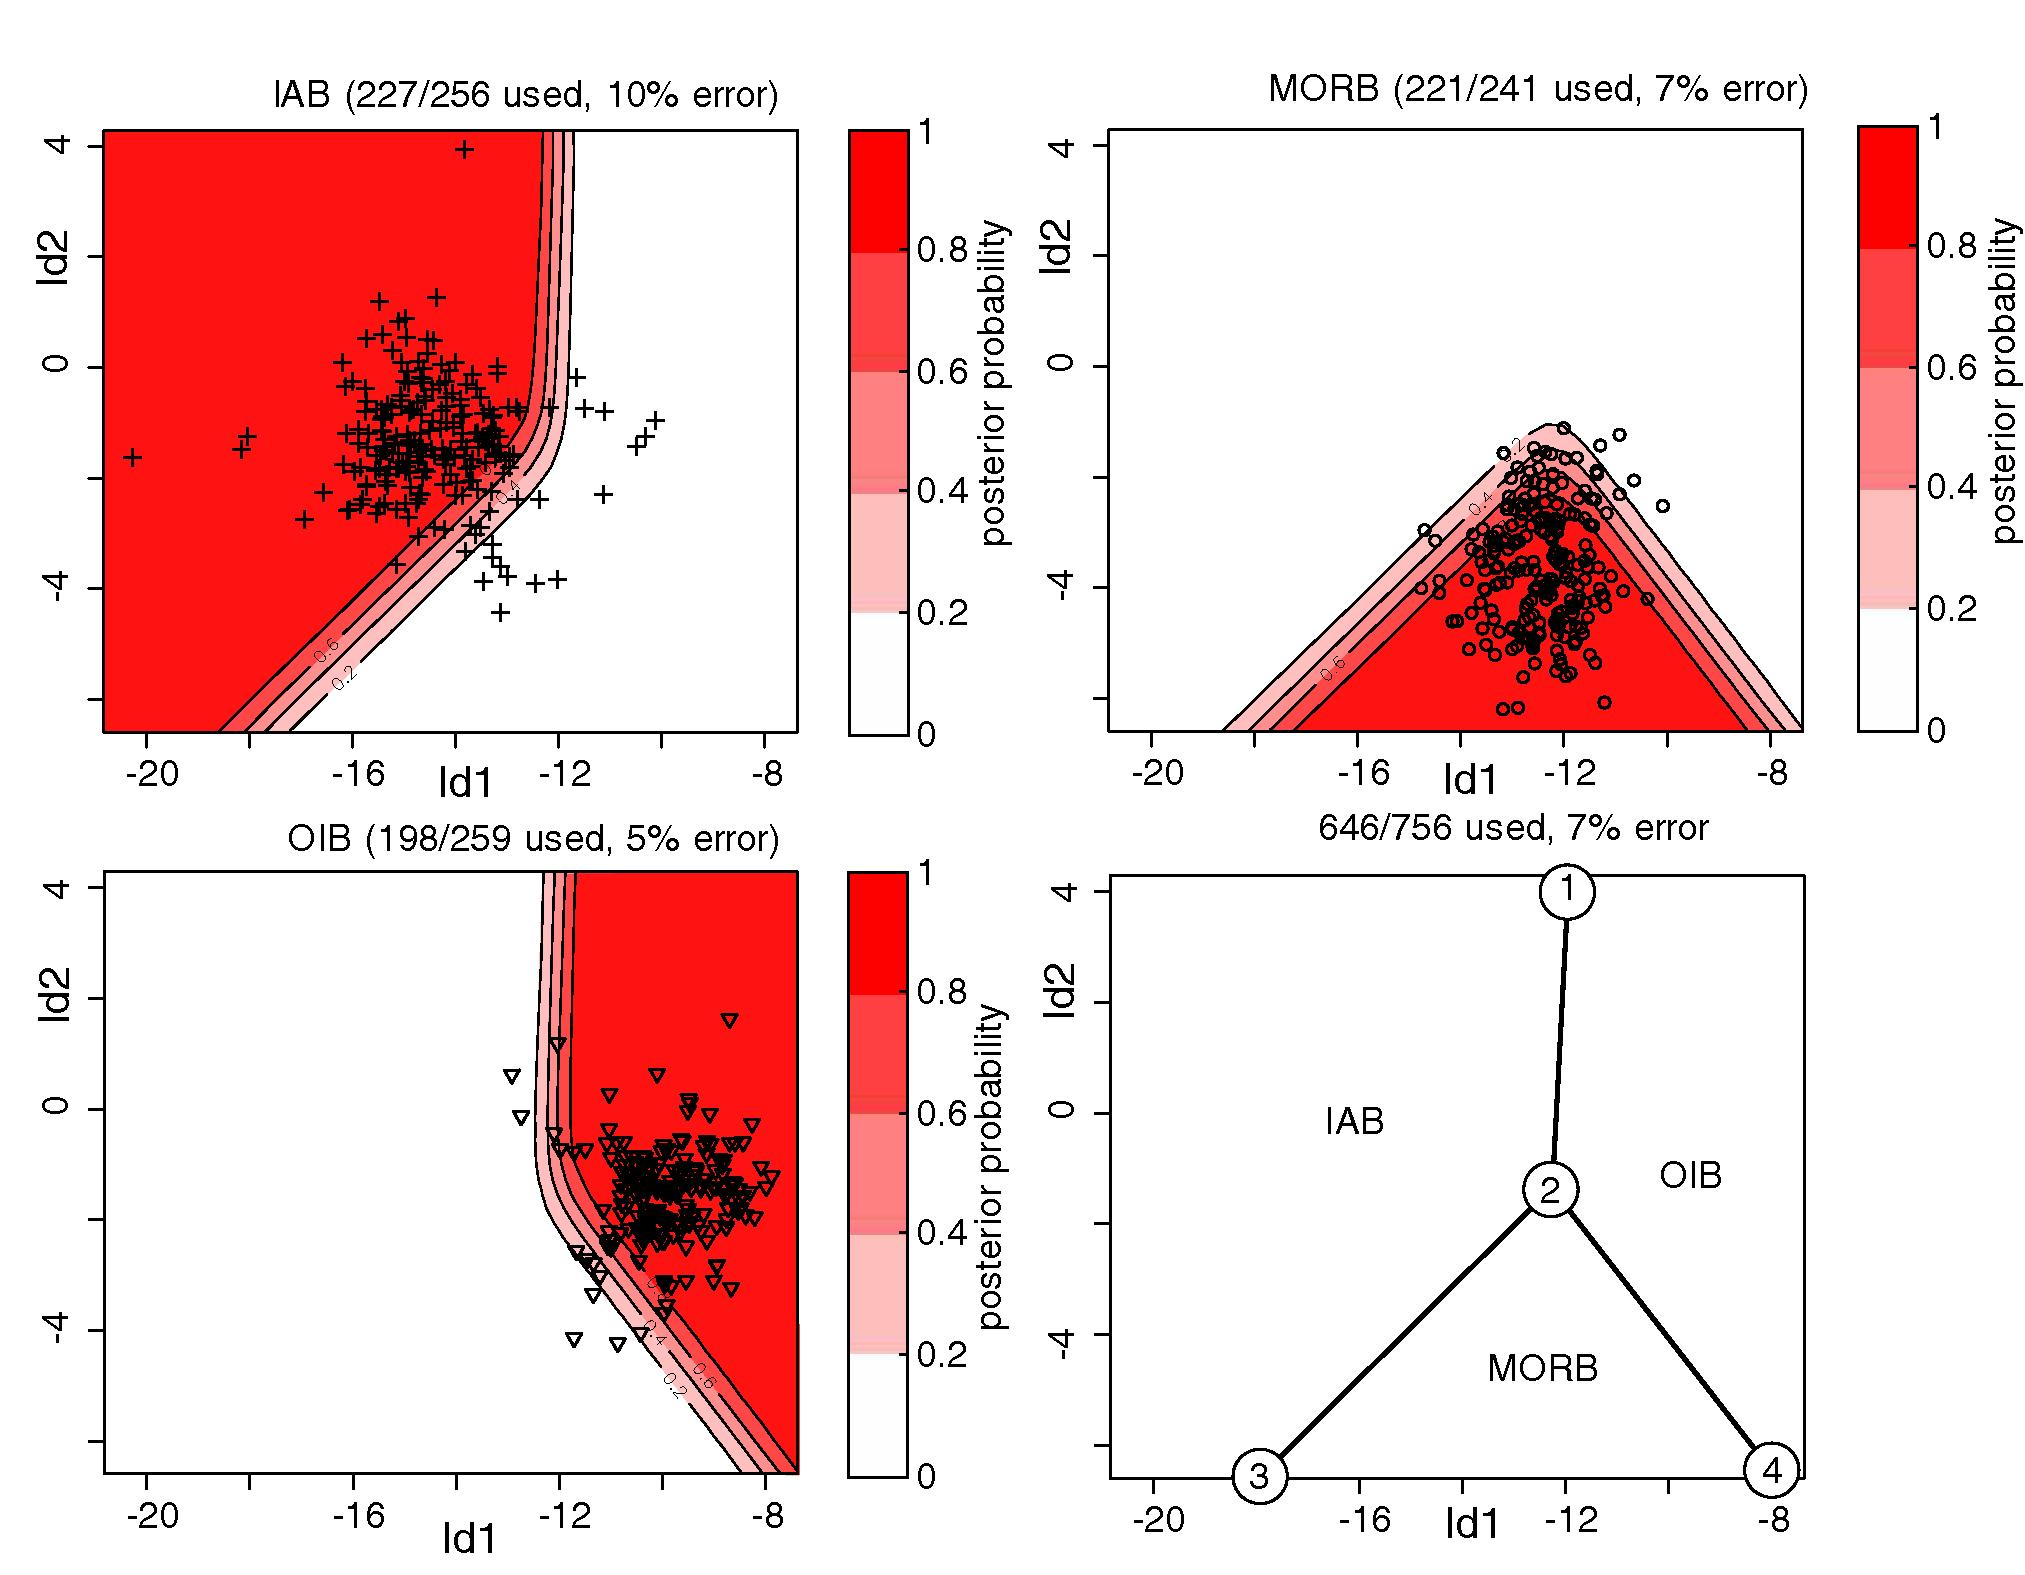
\includegraphics[width=600]{figures/discrimiFunc1.jpg}
  \caption[Linear discriminant analysis using major element data]{
Linear   discriminant  analysis  of   major  element   data  (SiO$_2$,
Al$_2$O$_3$,  TiO$_2$,  CaO, MgO,  MnO,  K$_2$O,  Na$_2$O), mapped  to
$\mathbb{R}^2$  using the  logratio  transformation. ld1  and ld2  are
given  by Equation  \ref{eq:ld_b}. Anchor  points are  given  in Table
\ref{tab:anchors}.}
  \label{fig:discrimiFunc2}
\end{figure}

\clearpage


\begin{figure}[htbp]
  \centering
  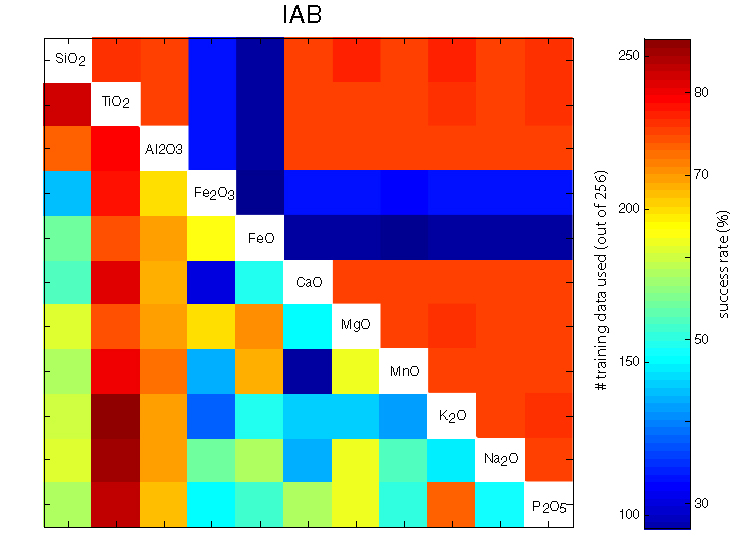
\includegraphics[width=300]{figures/xPlotMajor2_linear_IAB.jpg}
  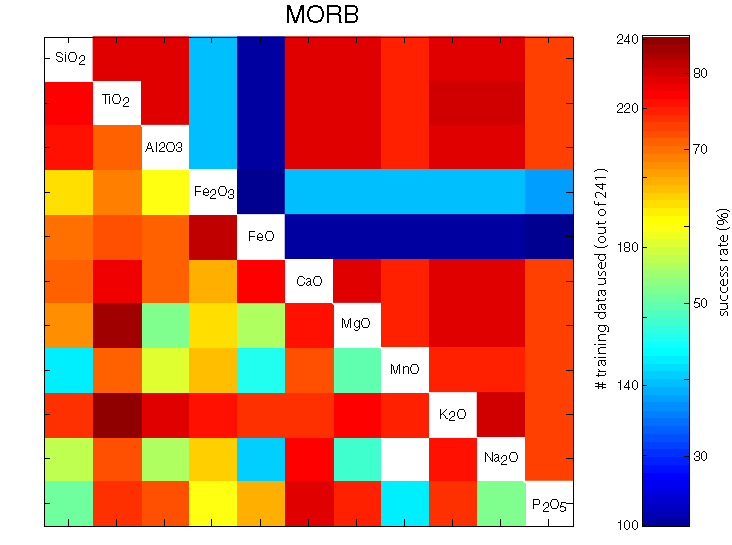
\includegraphics[width=300]{figures/xPlotMajor2_linear_MORB.jpg}\\
  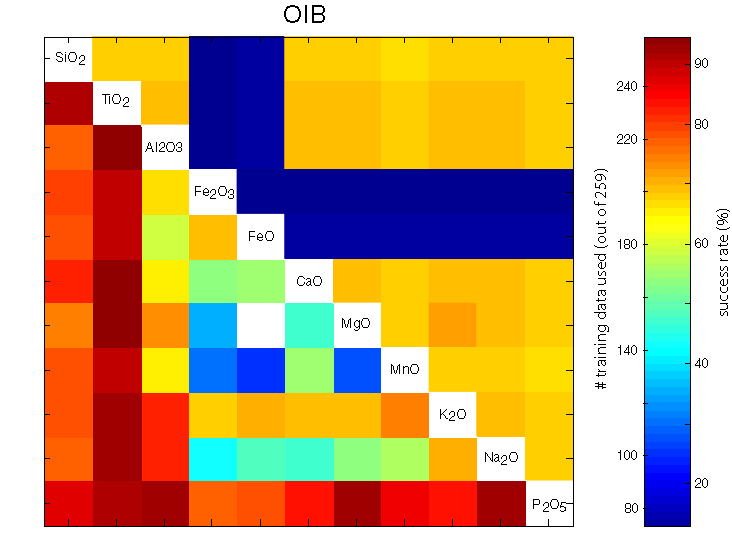
\includegraphics[width=300]{figures/xPlotMajor2_linear_OIB.jpg}
  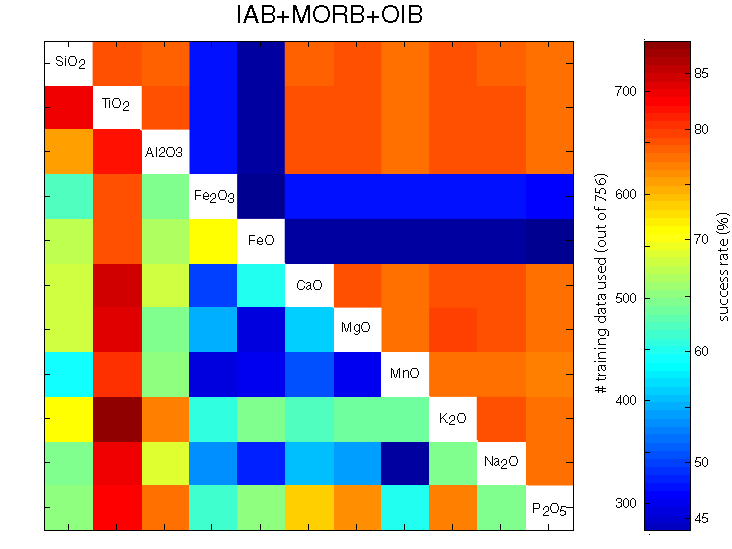
\includegraphics[width=300]{figures/xPlotMajor2_linear_err.jpg}
\caption[Exhaustive exploration of all bivariate linear discriminant 
analyses using only major elements]{
Visual  representation of  the performance  of all  possible bivariate
linear  discriminant analyses  using  the major  element  data of  the
training  set of  756  oceanic basalts.   The  upper right  triangular
section of each matrix shows the number of samples that contained both
variables.   The  lower  left  sections  color-code  the  fraction  of
successfully classified training data.}
  \label{fig:major2lin}
\end{figure}

\begin{figure}[htbp]
  \centering
  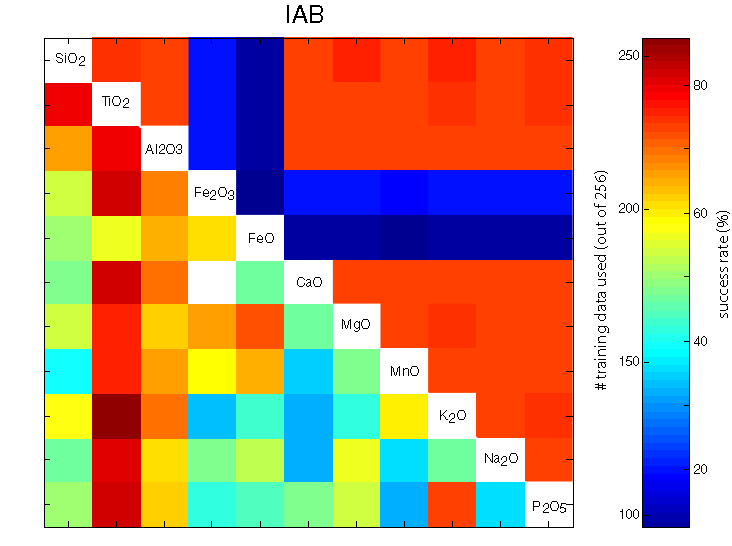
\includegraphics[width=300]{figures/xPlotMajor2_quadratic_IAB.jpg}
  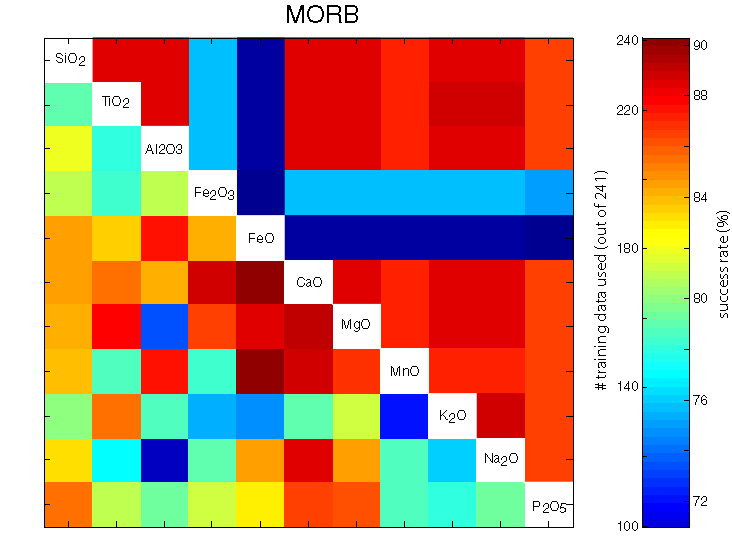
\includegraphics[width=300]{figures/xPlotMajor2_quadratic_MORB.jpg}\\
  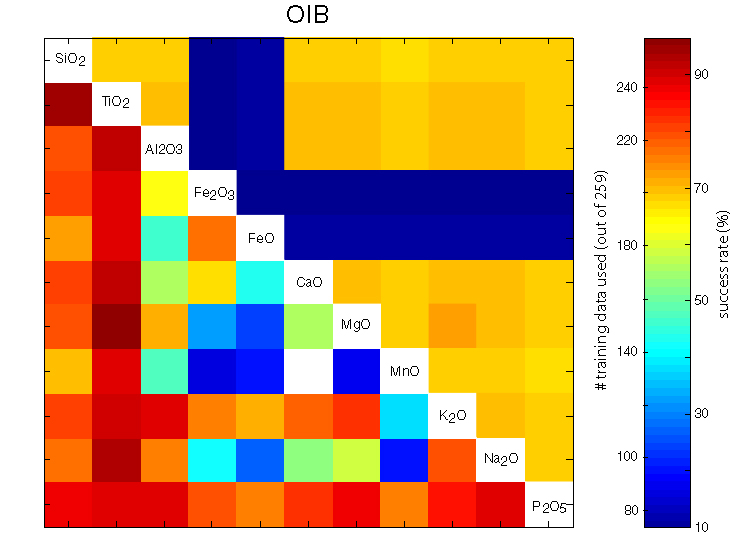
\includegraphics[width=300]{figures/xPlotMajor2_quadratic_OIB.jpg}
  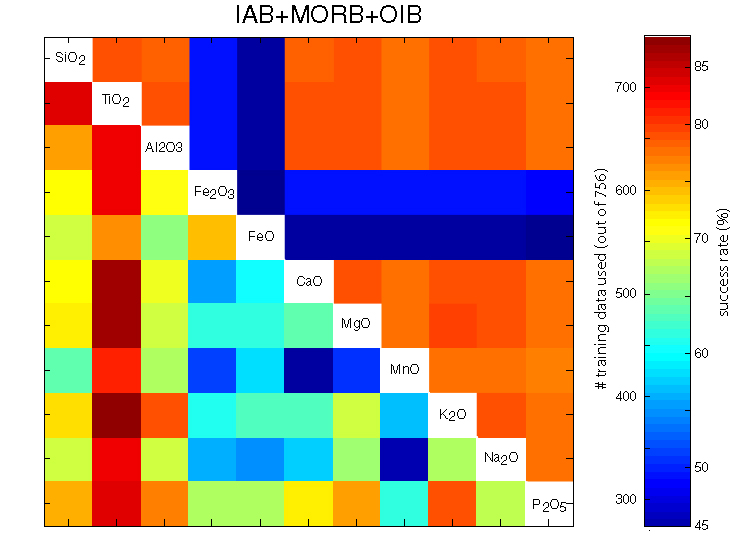
\includegraphics[width=300]{figures/xPlotMajor2_quadratic_err.jpg}
  \caption[Same  as Figure  \ref{fig:major2lin}, but  for
quadratic discriminant analysis]  {Same as Figure \ref{fig:major2lin},
but for quadratic discriminant analysis.}
  \label{fig:major2quad}
\end{figure}

\begin{figure}[htbp]
  \centering
  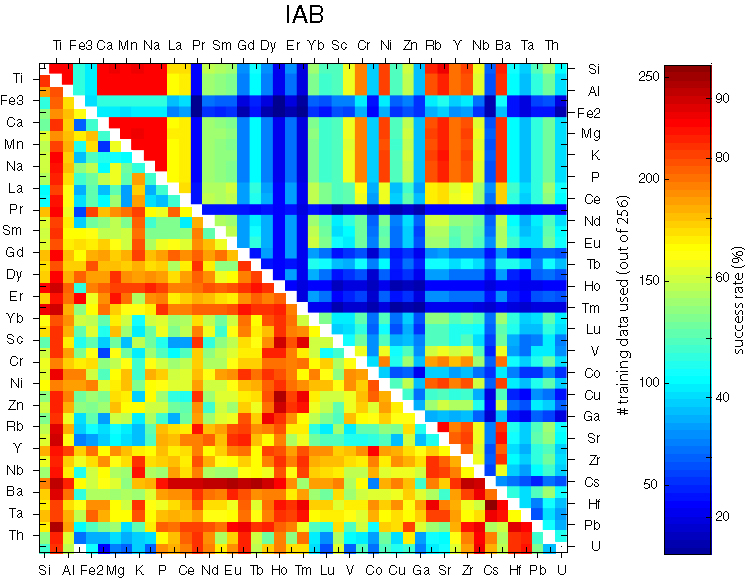
\includegraphics[width=300]{figures/xPlotTrace2_linear_IAB.jpg}
  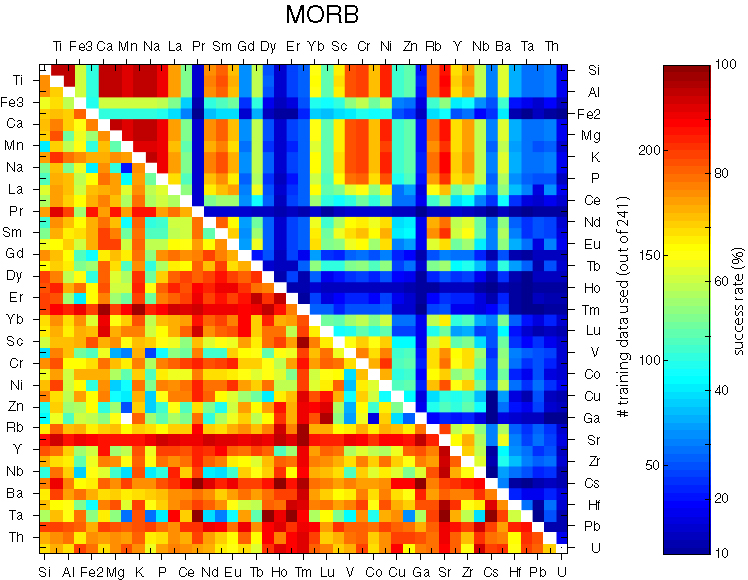
\includegraphics[width=300]{figures/xPlotTrace2_linear_MORB.jpg}\\
  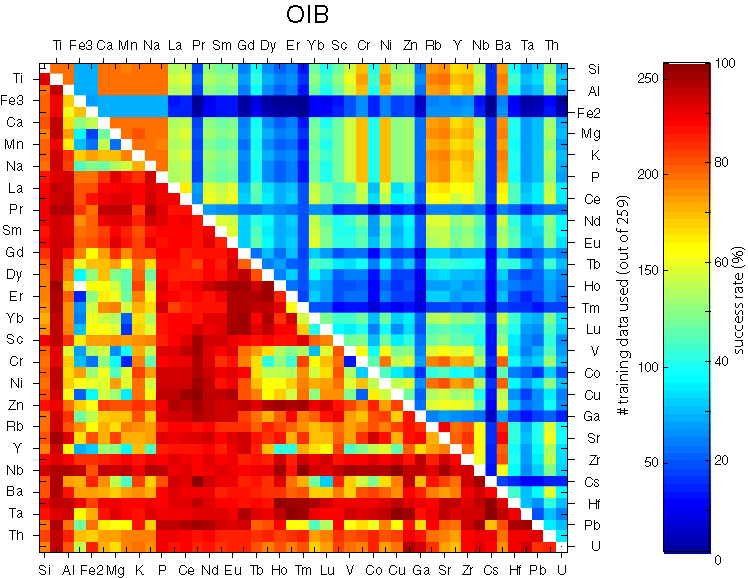
\includegraphics[width=300]{figures/xPlotTrace2_linear_OIB.jpg}
  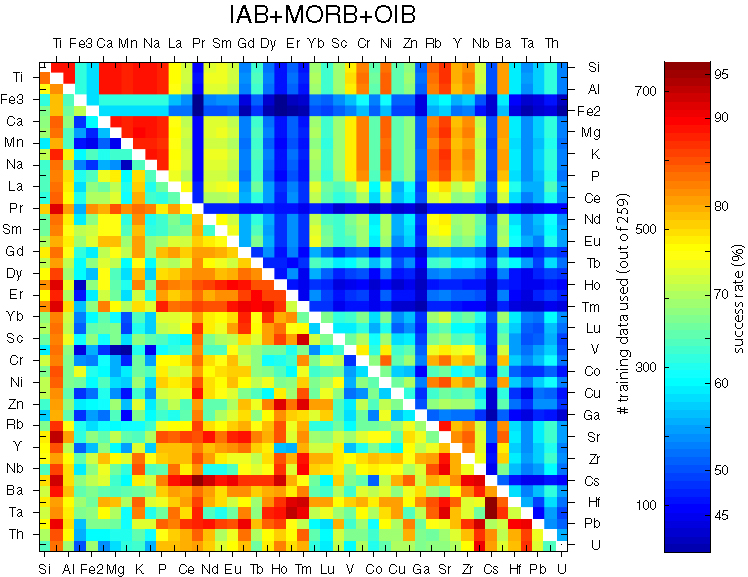
\includegraphics[width=300]{figures/xPlotTrace2_linear_err.jpg}
  \caption[Matrices   showing   the  performance   of   all  possible   bivariate
discriminant analyses using combinations of 45 elements]
{Matrices   showing   the  performance   of   all  possible   bivariate linear
discriminant analyses using combinations of 45 elements.}
  \label{fig:trace2lin}
\end{figure}

\begin{figure}[htbp]
  \centering
  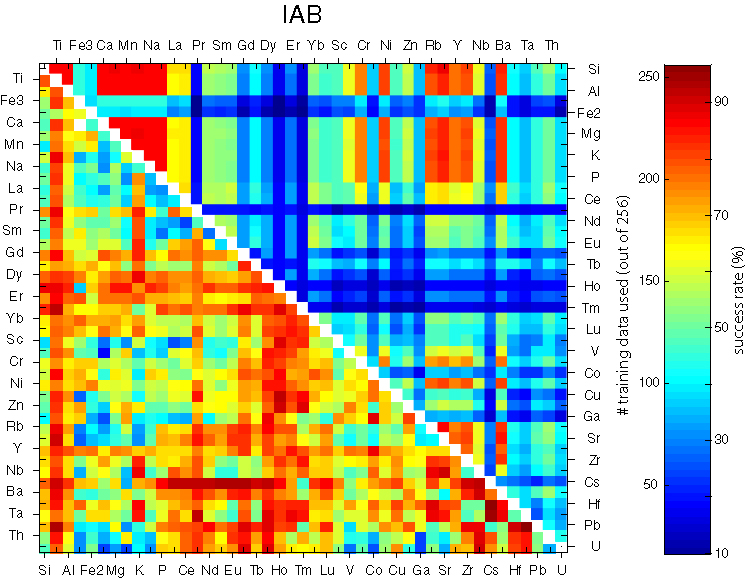
\includegraphics[width=300]{figures/xPlotTrace2_quadratic_IAB.jpg}
  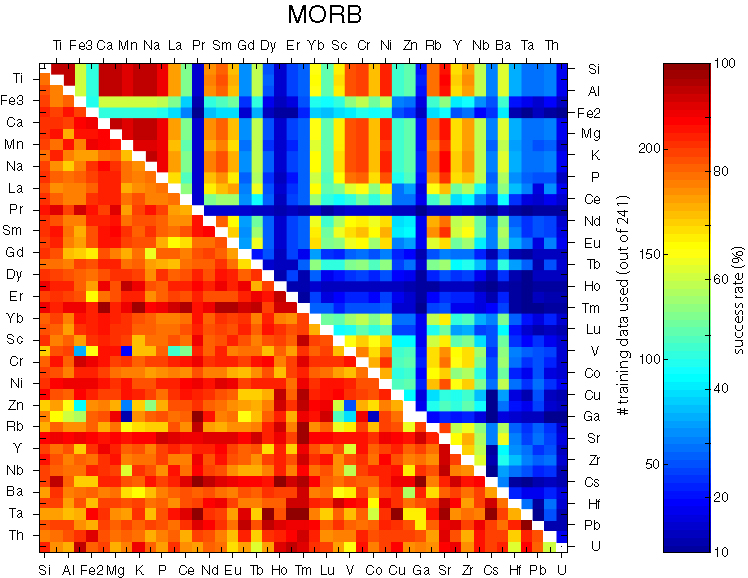
\includegraphics[width=300]{figures/xPlotTrace2_quadratic_MORB.jpg}\\
  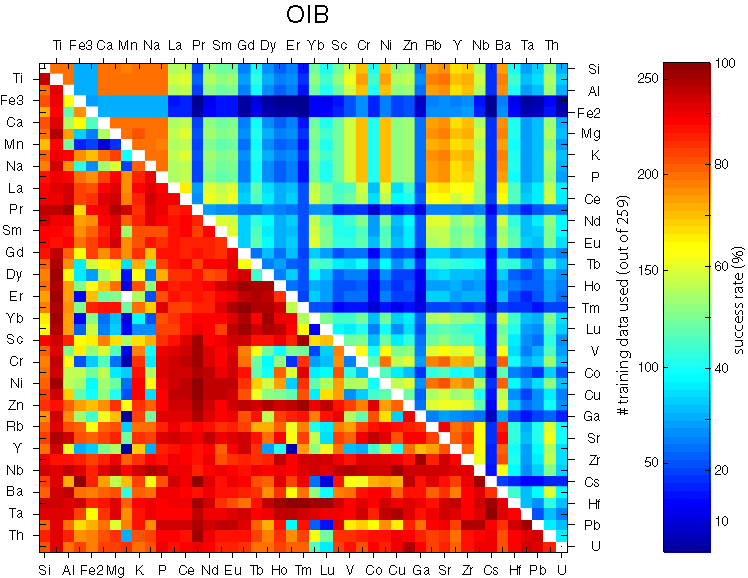
\includegraphics[width=300]{figures/xPlotTrace2_quadratic_OIB.jpg}
  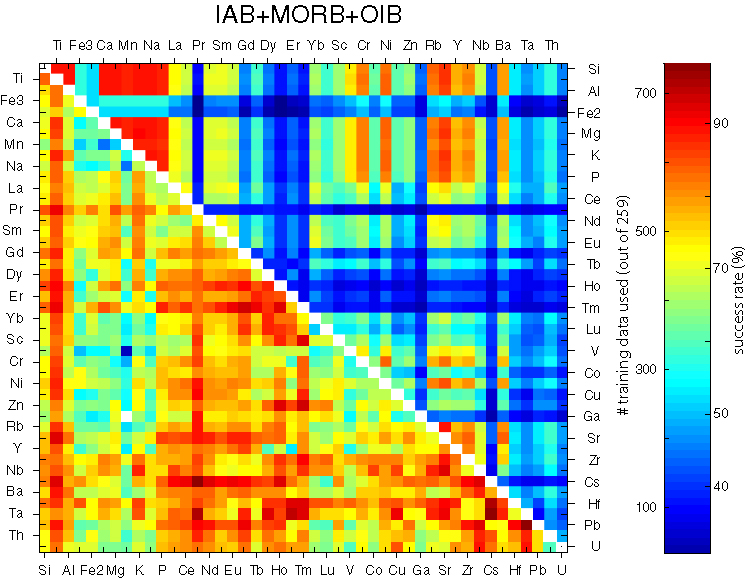
\includegraphics[width=300]{figures/xPlotTrace2_quadratic_err.jpg}
  \caption[Same  as Figure  \ref{fig:trace2lin}, but  for  quadratic discriminant analysis]
{Same  as Figure  \ref{fig:trace2lin}, but  for  quadratic discriminant analysis.}
  \label{fig:trace2quad}
\end{figure}

\clearpage

\begin{figure}[htbp]
  \centering
  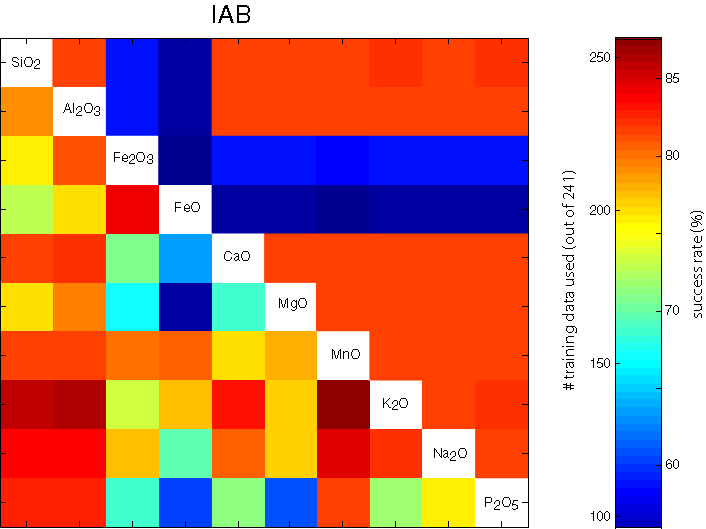
\includegraphics[width=300]{figures/xPlotMajor3Ti_linear_IAB.jpg}
  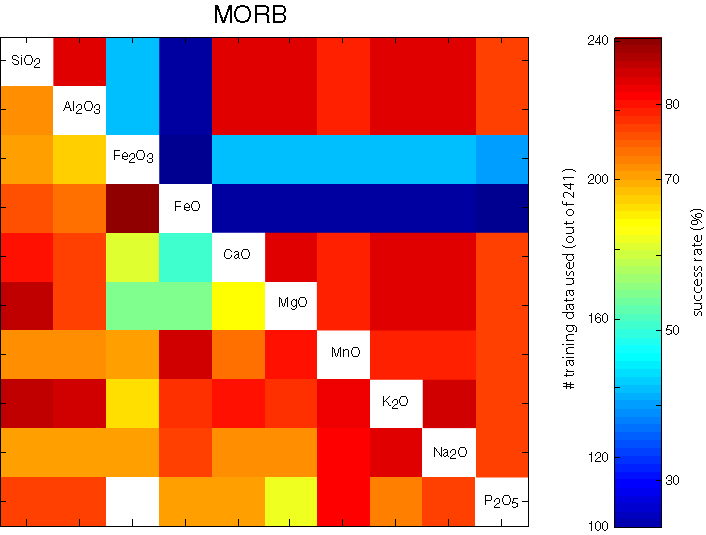
\includegraphics[width=300]{figures/xPlotMajor3Ti_linear_MORB.jpg}\\
  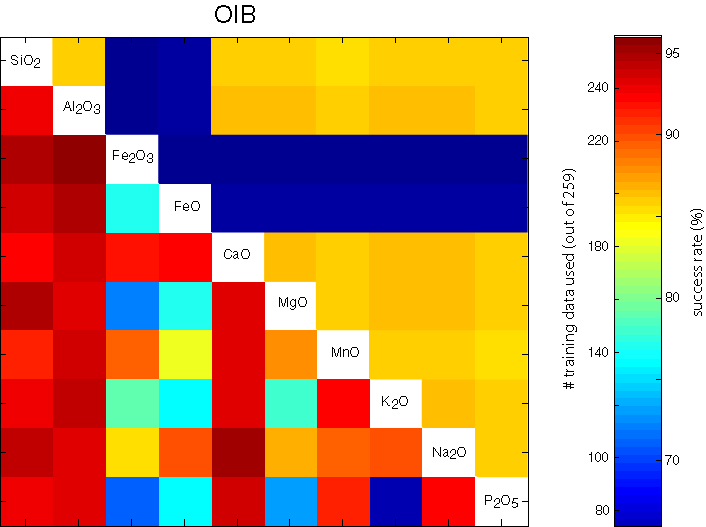
\includegraphics[width=300]{figures/xPlotMajor3Ti_linear_OIB.jpg}
  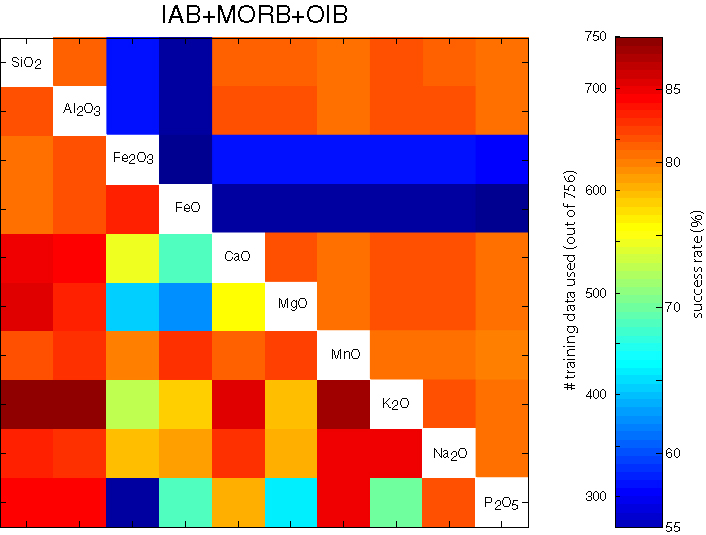
\includegraphics[width=300]{figures/xPlotMajor3Ti_linear_err.jpg}
  \caption[Performance  analysis of  all possible  ternary  discriminant analyses
 using TiO$_2$ and other major element oxides]
{Performance  analysis of  all possible  ternary  discriminant analyses
 using TiO$_2$ and other major element oxides.}
  \label{fig:major3lin}
\end{figure}

\begin{figure}[htbp]
  \centering
  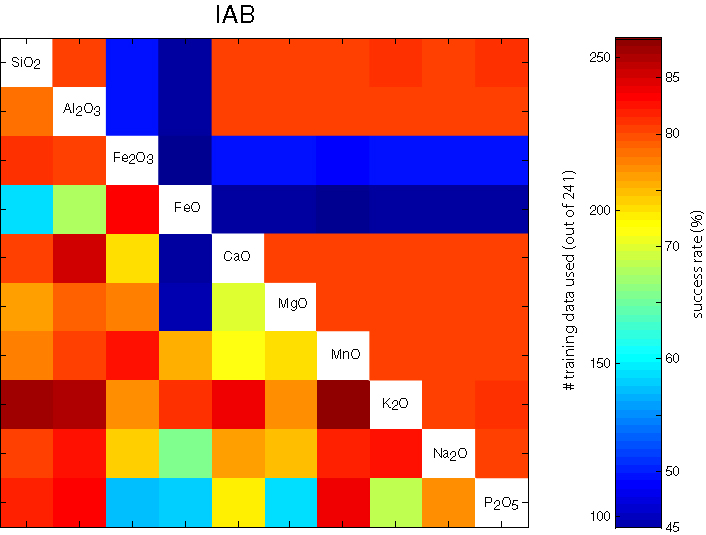
\includegraphics[width=300]{figures/xPlotMajor3Ti_quadratic_IAB.jpg}
  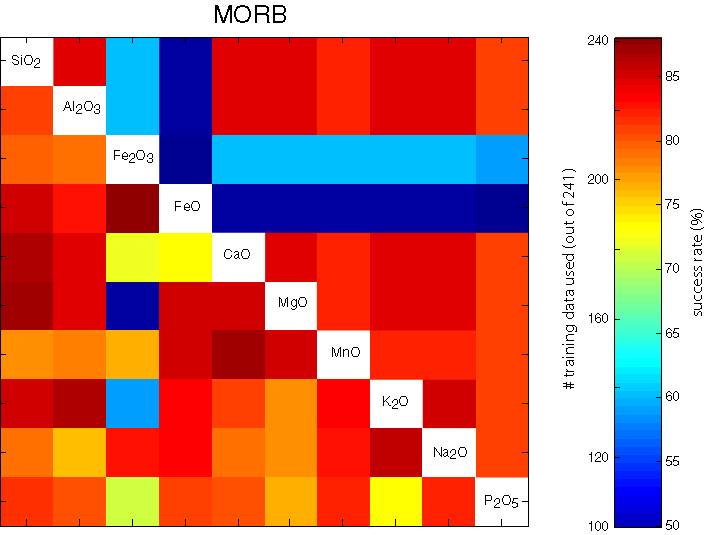
\includegraphics[width=300]{figures/xPlotMajor3Ti_quadratic_MORB.jpg}\\
  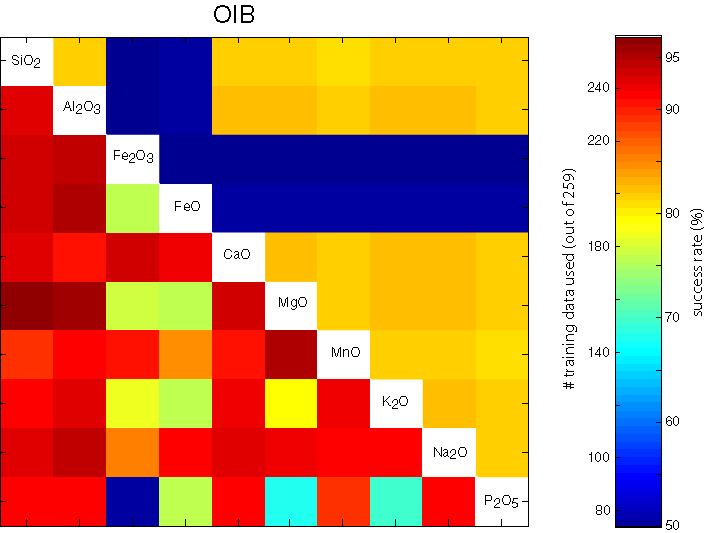
\includegraphics[width=300]{figures/xPlotMajor3Ti_quadratic_OIB.jpg}
  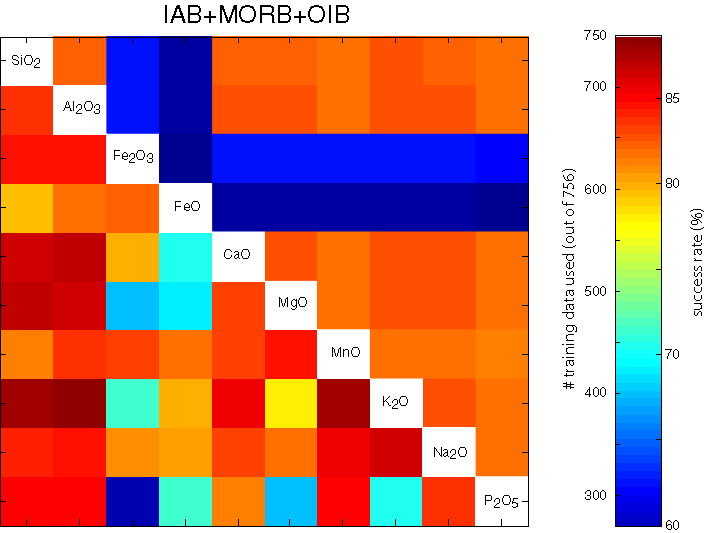
\includegraphics[width=300]{figures/xPlotMajor3Ti_quadratic_err.jpg}
  \caption[Same as  Figure \ref{fig:major3lin}, but  using quadratic discriminant analysis]
{Same as  Figure \ref{fig:major3lin}, but  using quadratic discriminant analysis.}
  \label{fig:major3quad}
\end{figure}

\begin{figure}[htbp]
  \centering
  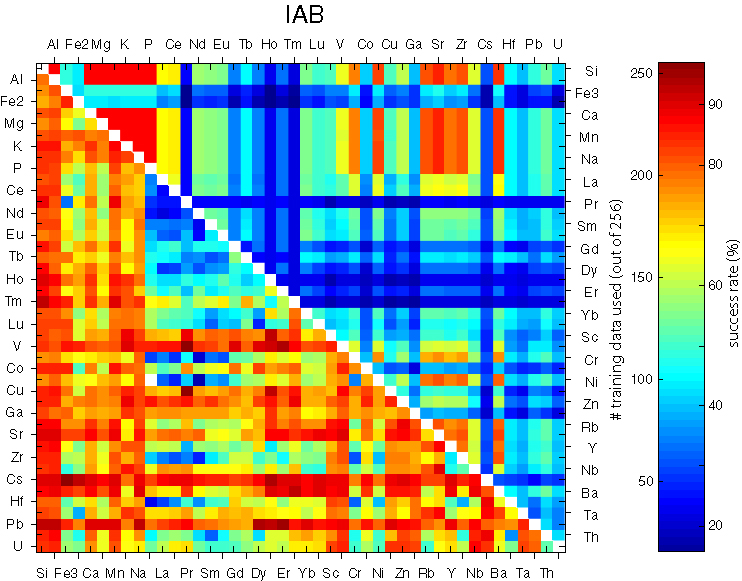
\includegraphics[width=300]{figures/xPlotTrace3Ti_linear_IAB.jpg}
  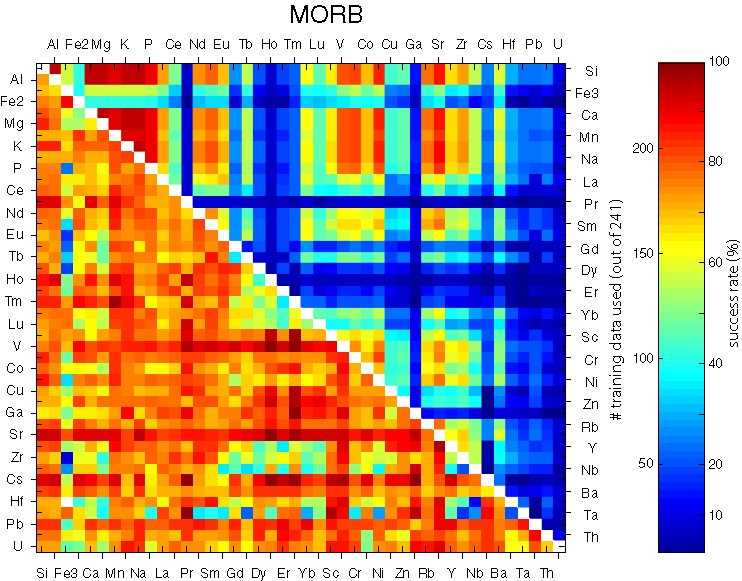
\includegraphics[width=300]{figures/xPlotTrace3Ti_linear_MORB.jpg}\\
  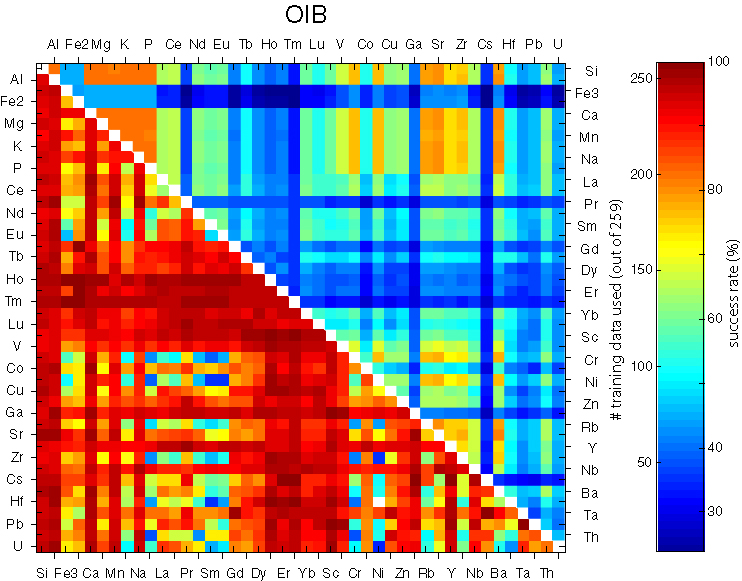
\includegraphics[width=300]{figures/xPlotTrace3Ti_linear_OIB.jpg}
  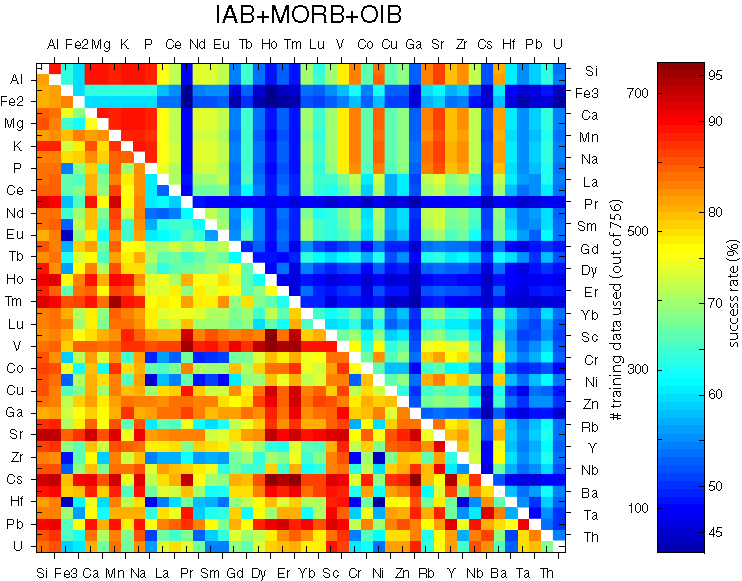
\includegraphics[width=300]{figures/xPlotTrace3Ti_linear_err.jpg}
  \caption[Performance  analysis of  all possible  ternary  discriminant analyses
using Ti and other elements]
{Performance  analysis of  all possible  ternary  discriminant analyses
using Ti and two of 45 other elements.}
  \label{fig:trace3lin}
\end{figure}

\begin{figure}[htbp]
  \centering
  \includegraphics[width=300]{figures/xPlotTrace3Ti_quadratic_IAB.jpg}
  \includegraphics[width=300]{figures/xPlotTrace3Ti_quadratic_MORB.jpg}\\
  \includegraphics[width=300]{figures/xPlotTrace3Ti_quadratic_OIB.jpg}
  \includegraphics[width=300]{figures/xPlotTrace3Ti_quadratic_err.jpg}
  \caption[Same as  Figure \ref{fig:trace3lin}, but  using quadratic discriminant analysis]
{Same as  Figure \ref{fig:trace3lin}, but  using quadratic discriminant analysis.}
  \label{fig:trace3quad}
\end{figure}

\clearpage

\begin{figure}[htbp]
  \centering
  \includegraphics[width=600]{figures/Si_Ti_Sr_lin.jpg}
  \caption[Best ternary linear discriminant analysis (using Si, Ti, and Sr)]{
The best ternary linear discriminant analysis, using Si, Ti, and Sr.}
  \label{fig:Si_Ti_Sr_lin}
\end{figure}

\begin{figure}[htbp]
  \centering
  \includegraphics[width=600]{figures/Eu_Lu_Sr_lin.jpg}
  \caption[Linear discriminant analysis using Eu, Lu, and Sr]
{Linear discriminant analysis using Eu, Lu, and Sr.}
  \label{fig:Eu_Lu_Sr_lin}
\end{figure}

\begin{figure}[htbp]
  \centering
  \includegraphics[width=600]{figures/V_Ti_Sc_lin.jpg}
  \caption[Linear discriminant analysis using Ti, V and Sc]
{The   best  performing  linear   discriminant  analysis   using  only
incompatible elements (Ti, V and Sc).}
  \label{fig:V_Ti_Sc_lin}
\end{figure}

\clearpage

\begin{figure}[htbp]
  \centering
  \includegraphics[width=600]{figures/Na_Nb_Sr_quad.jpg}
  \caption[Quadratic discriminant analysis using Na, Nb and Sr]
{The best performing quadratic discriminant analysis, using Na, Nb and
Sr.}
  \label{fig:Na_Nb_Sr_quad}
\end{figure}

\begin{figure}[htbp]
  \centering
  \includegraphics[width=600]{figures/V_Ti_Sm_quad.jpg}
  \caption[Quadratic discriminant analysis using Ti, V and Sm]
{The  best  performing  quadratic  discriminant  analysis  using  only
incompatible elements (Ti, V and Sm).}
  \label{fig:V_Ti_Sm_quad}
\end{figure}

\begin{figure}[htbp]
  \centering
  \includegraphics[width=500]{figures/biasVariance.jpg}
  \caption[Illustration of the bias-variance tradeoff in a regression context]
{Illustration of  the bias-variance tradeoff in  a regression context.
The thick gray  line is the true model (Y =  X$^4$). The white circles
are  50 samples with  random normal  errors.  The  dashed line  is the
interpolator,  which  is one  of  infinitely  many  functions that  go
through all the datapoints and,  thus, have zero bias. The solid black
line is  a linear regression model,  which has a large  bias but small
variance. In this case, the fourth order polynomial (blue) is the best
predictor of  future behavior.  Although  it has larger bias  than the
50th order polynomial  (red) and larger variance than  the first order
polynomial (straight black line),  it minimizes the mean squared error
(MSE = variance + bias$^2$).}
  \label{fig:biasVariance}
\end{figure}

\begin{figure}[htbp]
  \centering
a.  \includegraphics[width=300]{figures/Shervais.jpg}\\
b.  \includegraphics[width=300]{figures/log_Ti_V_lin.jpg}
c.  \includegraphics[width=300]{figures/log_Ti_V_q.jpg}
d.  \includegraphics[width=300]{figures/test_Ti_V_lin.jpg}
e.  \includegraphics[width=300]{figures/test_Ti_V_q.jpg}
  \caption[The test data plotted on various versions of the Ti-V diagram]
{The test data (116/182 used)  plotted on various versions of the Ti-V
diagram with: a. the  original decision boundaries of Shervais (1982),
drawn by  eye; b.   LDA on the  logratio-plot, with anchor  points 1-4
given in Table \ref{tab:anchors}; c.  QDA on the logratio-plot, d. the
same  LDA  as  in  subplot  b.,  but this  time  mapped  back  to  the
``traditional''  compositional  data space;  e.   the  QDA of  subplot
c.  mapped  back  to  Ti-V  space.  An error  analysis  of  these  and
subsequent   diagrams  is   given  in   Tables   \ref{tab:errEst}  and
\ref{tab:comparison}.}
  \label{fig:log_Ti_V}
\end{figure}

\begin{figure}[htbp]
  \centering
a.  \includegraphics[width=300]{figures/PearceTiZr.jpg}\\
b.  \includegraphics[width=300]{figures/log_Ti_Zr_lin.jpg}
c.  \includegraphics[width=300]{figures/log_Ti_Zr_q.jpg}
d.  \includegraphics[width=300]{figures/test_Ti_Zr_lin.jpg}
e.  \includegraphics[width=300]{figures/test_Ti_Zr_q.jpg}
  \caption[The test data plotted on the Ti-Zr diagram]
{The test data (89/182 used) plotted on the Ti-Zr diagram with: a. the
original  decision boundaries  of Pearce  and Cann  (1973); b-e  as in
Figure \ref{fig:log_Ti_V}.}
  \label{fig:log_Ti_Zr}
\end{figure}

\begin{figure}[htbp]
  \centering
a.  \includegraphics[width=300]{figures/PearceTiZrY.jpg}\\
b.  \includegraphics[width=300]{figures/log_Ti_Zr_Y_lin.jpg}
c.  \includegraphics[width=300]{figures/log_Ti_Zr_Y_q.jpg}
d.  \includegraphics[width=300]{figures/test_Ti_Zr_Y_lin.jpg}
e.  \includegraphics[width=300]{figures/test_Ti_Zr_Y_q.jpg}
  \caption[The test data plotted on the Ti-Zr-Y diagram]{
The  test data  (85/182 used)  plotted  on the  Ti-Zr-Y diagram  with:
a. the original decision boundaries  of Pearce and Cann (1973); b-e as
in Figure \ref{fig:log_Ti_V}.}
  \label{fig:log_Ti_Zr_Y}
\end{figure}

\begin{figure}[htbp]
  \centering
a.  \includegraphics[width=300]{figures/Meschede.jpg}\\
b.  \includegraphics[width=300]{figures/log_Nb_Zr_Y_lin.jpg}
c.  \includegraphics[width=300]{figures/log_Nb_Zr_Y_q.jpg}
d.  \includegraphics[width=300]{figures/test_Nb_Zr_Y_lin.jpg}
e.  \includegraphics[width=300]{figures/test_Nb_Zr_Y_q.jpg}
  \caption[The test data plotted on the Nb-Zr-Y diagram]
{The test data  (58/182 used) plotted on the  Nb-Zr-Y diagram with: a.
the original decision boundaries of  Meschede (1986); b-e as in Figure
\ref{fig:log_Ti_V}.}
  \label{fig:log_Nb_Zr_Y}
\end{figure}

\begin{figure}[htbp]
  \centering
a.  \includegraphics[width=300]{figures/Wood.jpg}\\
b.  \includegraphics[width=300]{figures/log_Th_Ta_Hf_lin.jpg}
c.  \includegraphics[width=300]{figures/log_Th_Ta_Hf_q.jpg}
d.  \includegraphics[width=300]{figures/test_Th_Ta_Hf_lin.jpg}
e.  \includegraphics[width=300]{figures/test_Th_Ta_Hf_q.jpg}
  \caption[The test data plotted on the Th-Ta-Hf diagram]
{The test  data (36/182 used, but  no MORBs!) plotted  on the Th-Ta-Hf
diagram with: a. the original  decision boundaries of Wood (1980); b-e
as in Figure \ref{fig:log_Ti_V}.}
  \label{fig:log_Th_Ta_Hf}
\end{figure}

\begin{figure}[htbp]
  \centering
a.  \includegraphics[width=300]{figures/log_Si_Ti_Sr_lin.jpg}
b.  \includegraphics[width=300]{figures/test_Si_Ti_Sr_lin.jpg}
  \caption[The test data plotted on the Si-Ti-Sr diagram]
{The  test data  (164/182 used)  plotted on  the Si-Ti-Sr  LDA diagram
with:  a.   the  decision  boundaries  and anchor  points  (see  Table
\ref{tab:anchors})  in log-ratio  space; b.   the  decision boundaries
mapped back to the simplex.}
  \label{fig:log_Si_Ti_Sr}
\end{figure}

\begin{figure}[htbp]
  \centering
a.  \includegraphics[width=300]{figures/log_Eu_Lu_Sr_lin.jpg}
b.  \includegraphics[width=300]{figures/test_Eu_Lu_Sr_lin.jpg}
  \caption[The test data plotted on the Eu-Lu-Sr diagram]
{The test data (103/182 used)  plotted on the Eu-Lu-Sr LDA diagram;  a
\& b as in Figure \ref{fig:log_Si_Ti_Sr}.}
  \label{fig:log_Eu_Lu_Sr}
\end{figure}

\begin{figure}[htbp]
  \centering
a.  \includegraphics[width=300]{figures/log_V_Ti_Sc_lin.jpg}
b.  \includegraphics[width=300]{figures/test_V_Ti_Sc_lin.jpg}
  \caption[The test data plotted on the Ti-V-Sc diagram]
{The test data (72/182 used) plotted on the Ti-V-Sc LDA diagram;  a \&
b as in Figure \ref{fig:log_Si_Ti_Sr}.}
  \label{fig:log_V_Ti_Sc}
\end{figure}

\begin{figure}[htbp]
  \centering
a.  \includegraphics[width=300]{figures/log_Na_Nb_Sr_q.jpg}
b.  \includegraphics[width=300]{figures/test_Na_Nb_Sr_q.jpg}
  \caption[The test data plotted on the Na-Nb-Sr diagram]
{The test data (61/182 used) plotted on the Na-Nb-Sr QDA diagram with:
a.   the decision  boundaries in  log-ratio space;  b. mapped  back to
$\Delta_2$.}
  \label{fig:log_Na_Nb_Sr}
\end{figure}

\begin{figure}[htbp]
  \centering
a.  \includegraphics[width=300]{figures/log_Ti_V_Sm_q.jpg}
b.  \includegraphics[width=300]{figures/test_Ti_V_Sm_q.jpg}
  \caption[The test data plotted on the Ti-V-Sm diagram]
{The test data (85/182 used) plotted on the Ti-V-Sm QDA diagram;  a \&
b as in Figure \ref{fig:log_Na_Nb_Sr}.}
  \label{fig:log_Ti_V_Sm}
\end{figure}
